\section{Contextualização} % (fold)
\label{sec:contextualizacao}

\begin{frame}
    Sistemas com vários itens ou serviços utilizam sistemas
de recomedação. Exemplo:
    \begin{itemize}
        \item Netflix
        \item Amazon
    \end{itemize}
\end{frame}

\begin{frame}
    \begin{itemize}
        \item O Debian possui mais de 49 mil pacotes
        \item A recomendação de pacotes pode ajudar o usuário
        na realização de suas atividades
    \end{itemize}
\end{frame}

% section what_is_solid_ (end)

\section{Problemática} % (fold)
\label{sec:problematica}

\begin{frame}
  \begin{itemize}
    \item Melhorar um sistema de recomendação
    \item Utilizar o contexto temporal
  \end{itemize}
\end{frame}

% section s (end)

\section{Objetivo} % (fold)
\label{sec:objetivo}

\begin{frame}
  \begin{itemize}
    \item Utilizar o contexto temporal para criar recomendações
    \item Estratégia determinística
    \item Aprendizado de máquina
  \end{itemize}
\end{frame}

% section o (end)

\section{Sistemas de recomendação} % (fold)
\label{sec:sistemas_recomendacao}
\begin{frame}
    \say {\textit{Sistemas de recomendação são ferramentas computacionais e
técnicas usadas para produzir recomendação de itens úteis a um
usuário}},\\(MAHMOOD; RICCI, 2009)
\end{frame}

\begin{frame}

\begin{figure}[h!]
  \centering
    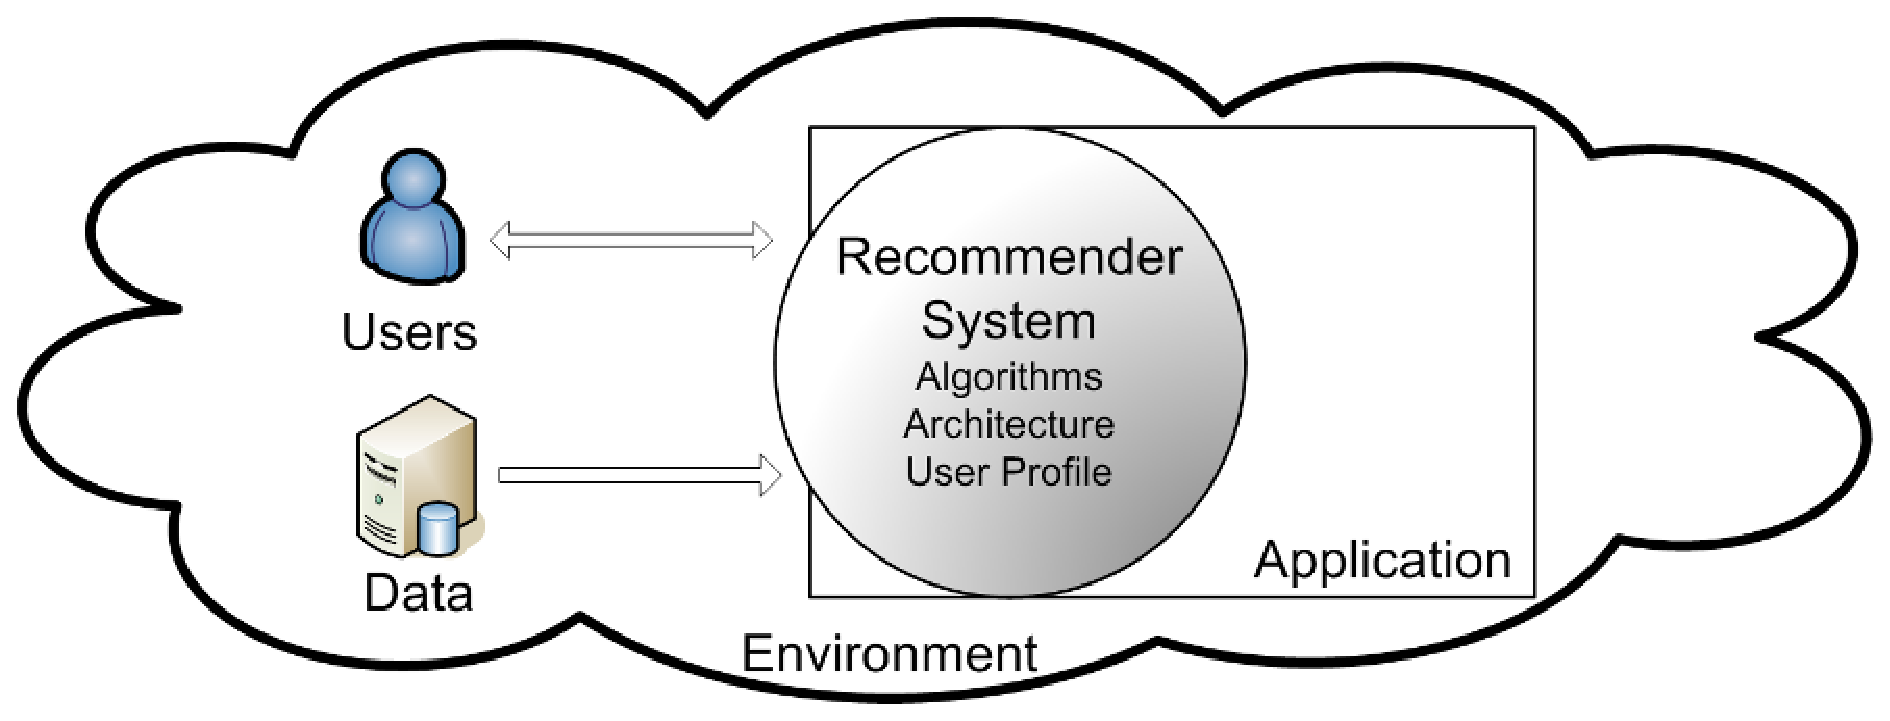
\includegraphics[width=1\textwidth]{figura/recommender_model.eps}
  \caption{Modelo para criação de um sistema de recomendação personalizado (PICAULT et al., 2011)}
\end{figure}

\end{frame}

\begin{frame}
    Tipos de sistemas de recomendação:

    \begin{itemize}
        \item Recomendação baseada em conteúdo
        \item Recomendação colaborativa
        \item Recomendação híbrida
        \item Recomendação por contexto
    \end{itemize}
\end{frame}

\begin{frame}

\begin{figure}[h!]
  \centering
    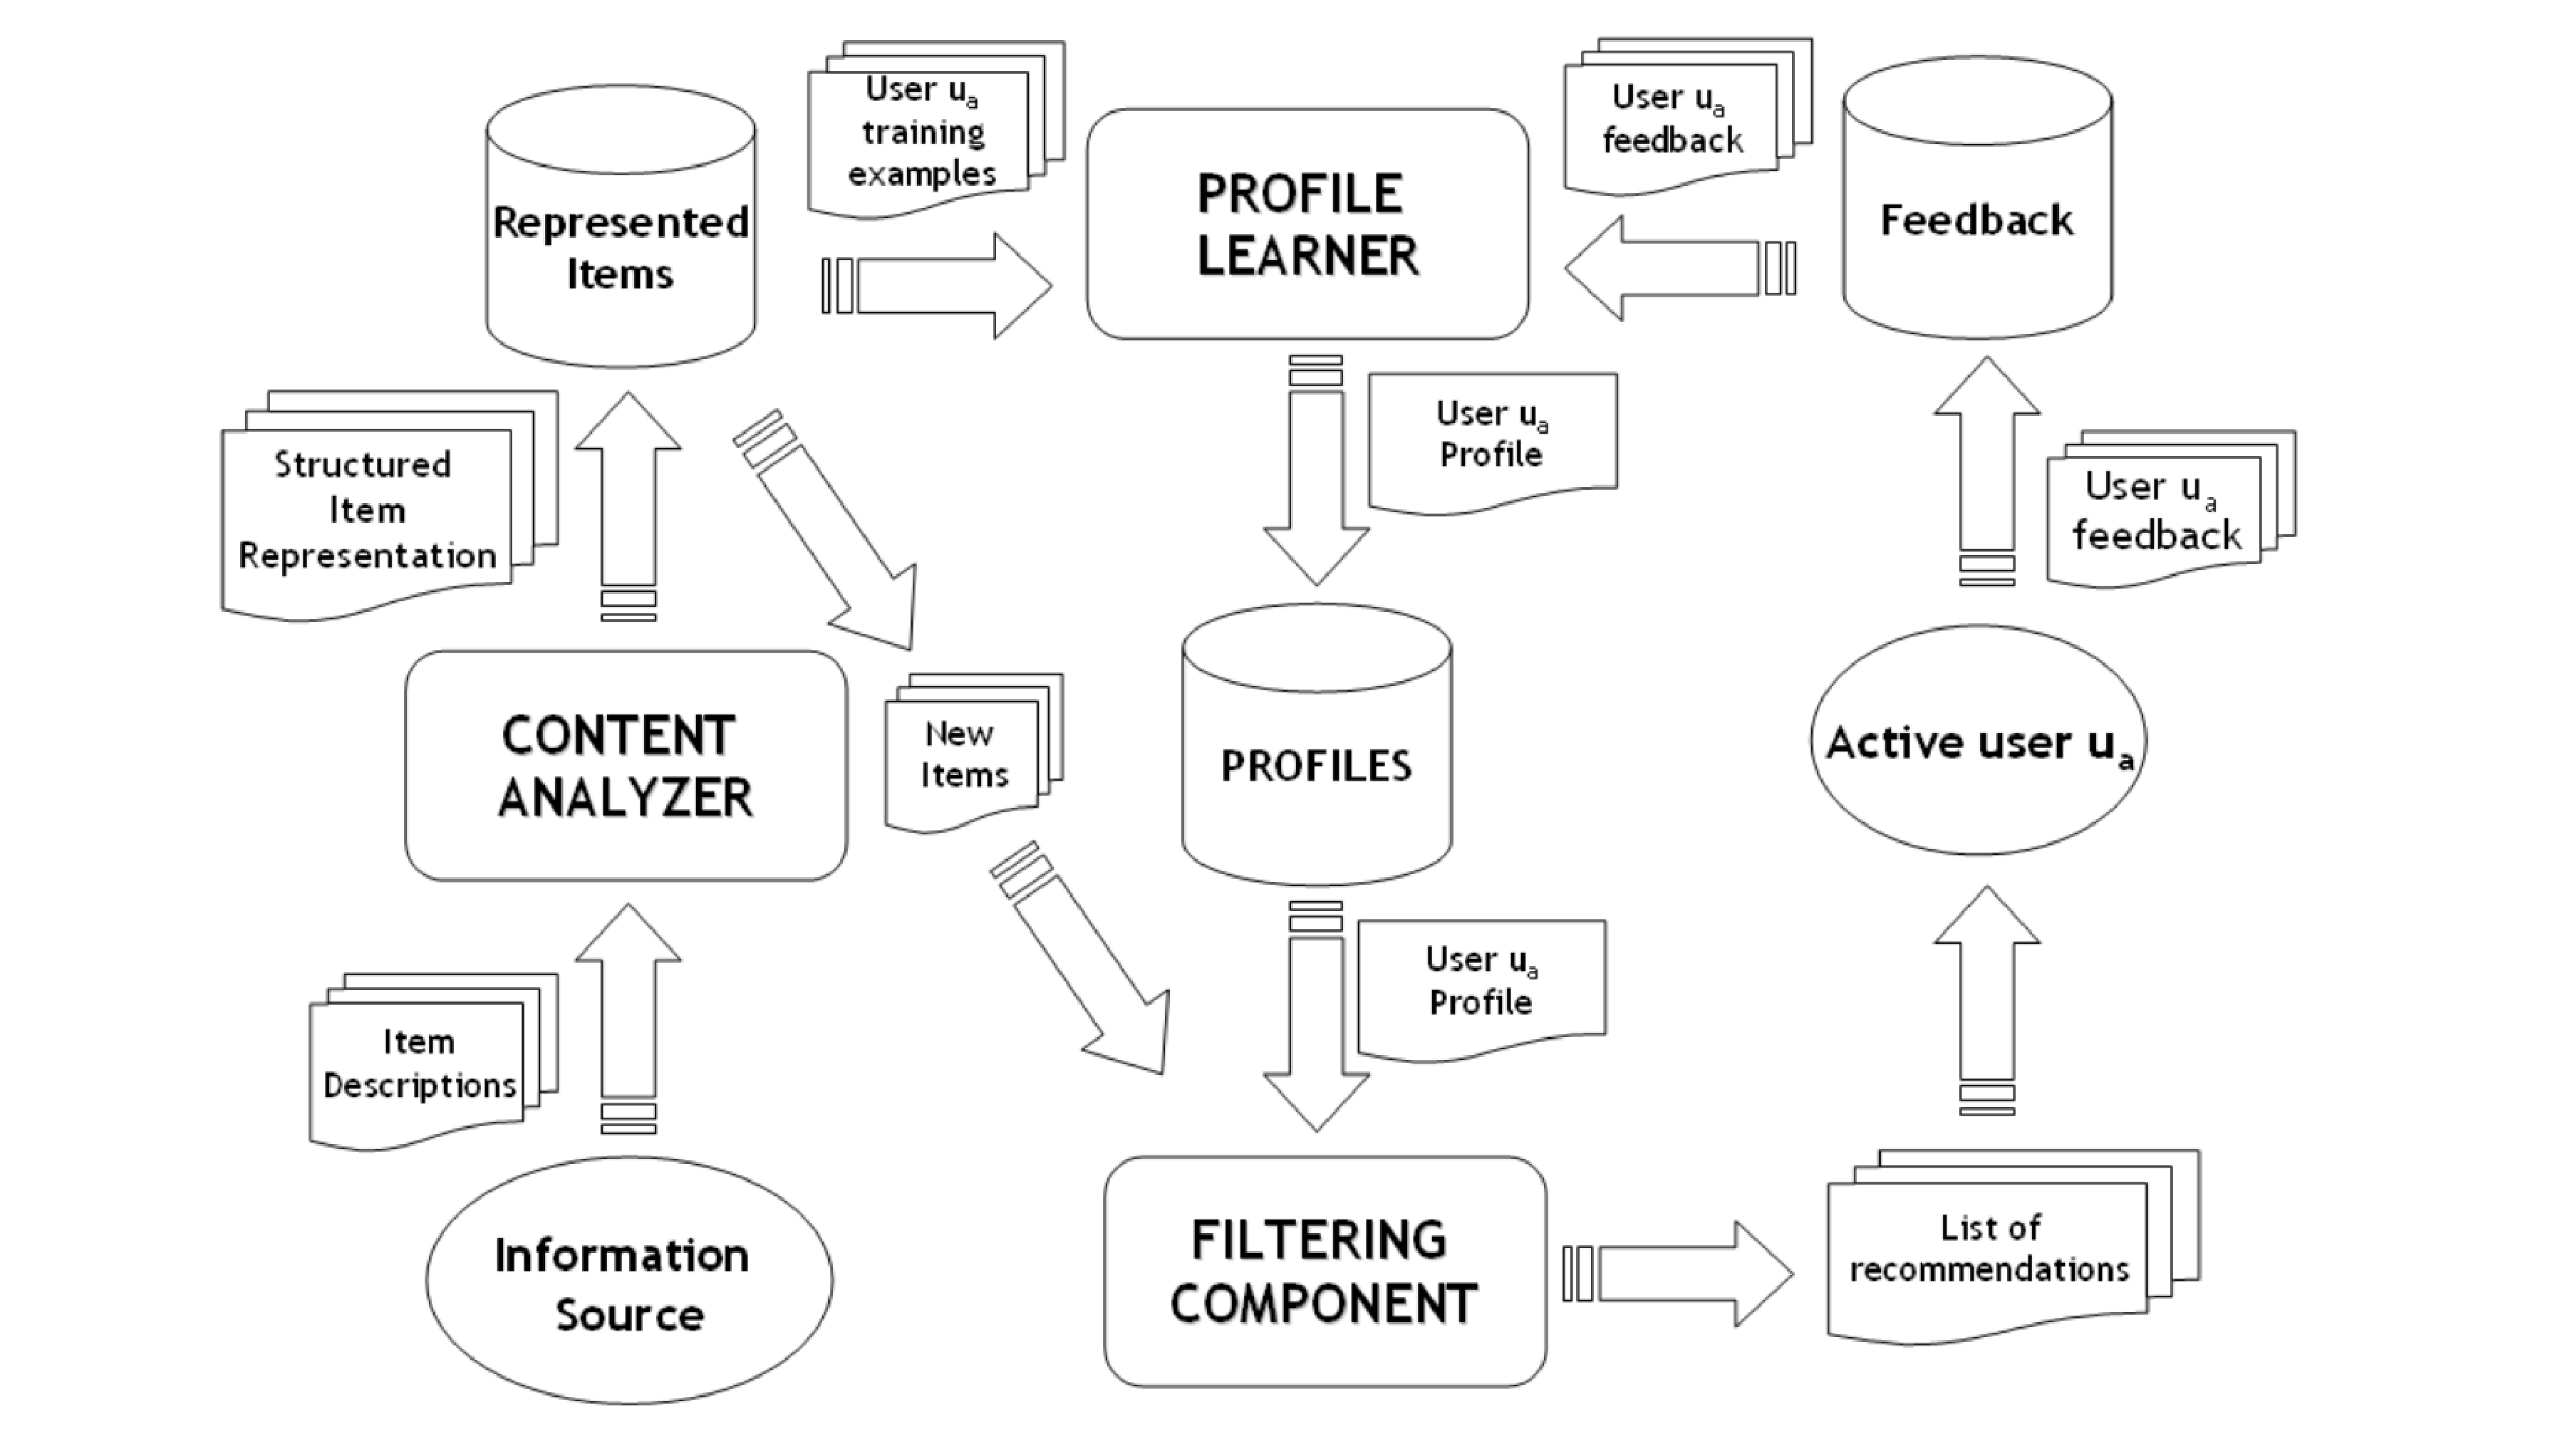
\includegraphics[width=1\textwidth]{figura/recomendacao_conteudo.eps}
  \caption{Fluxo para construção de um sistema de recomendação por conteúdo (LOPS; GEMMIS; SEMERARO, 2011)}
\end{figure}

\end{frame}

\begin{frame}

\begin{figure}[h!]
  \centering
    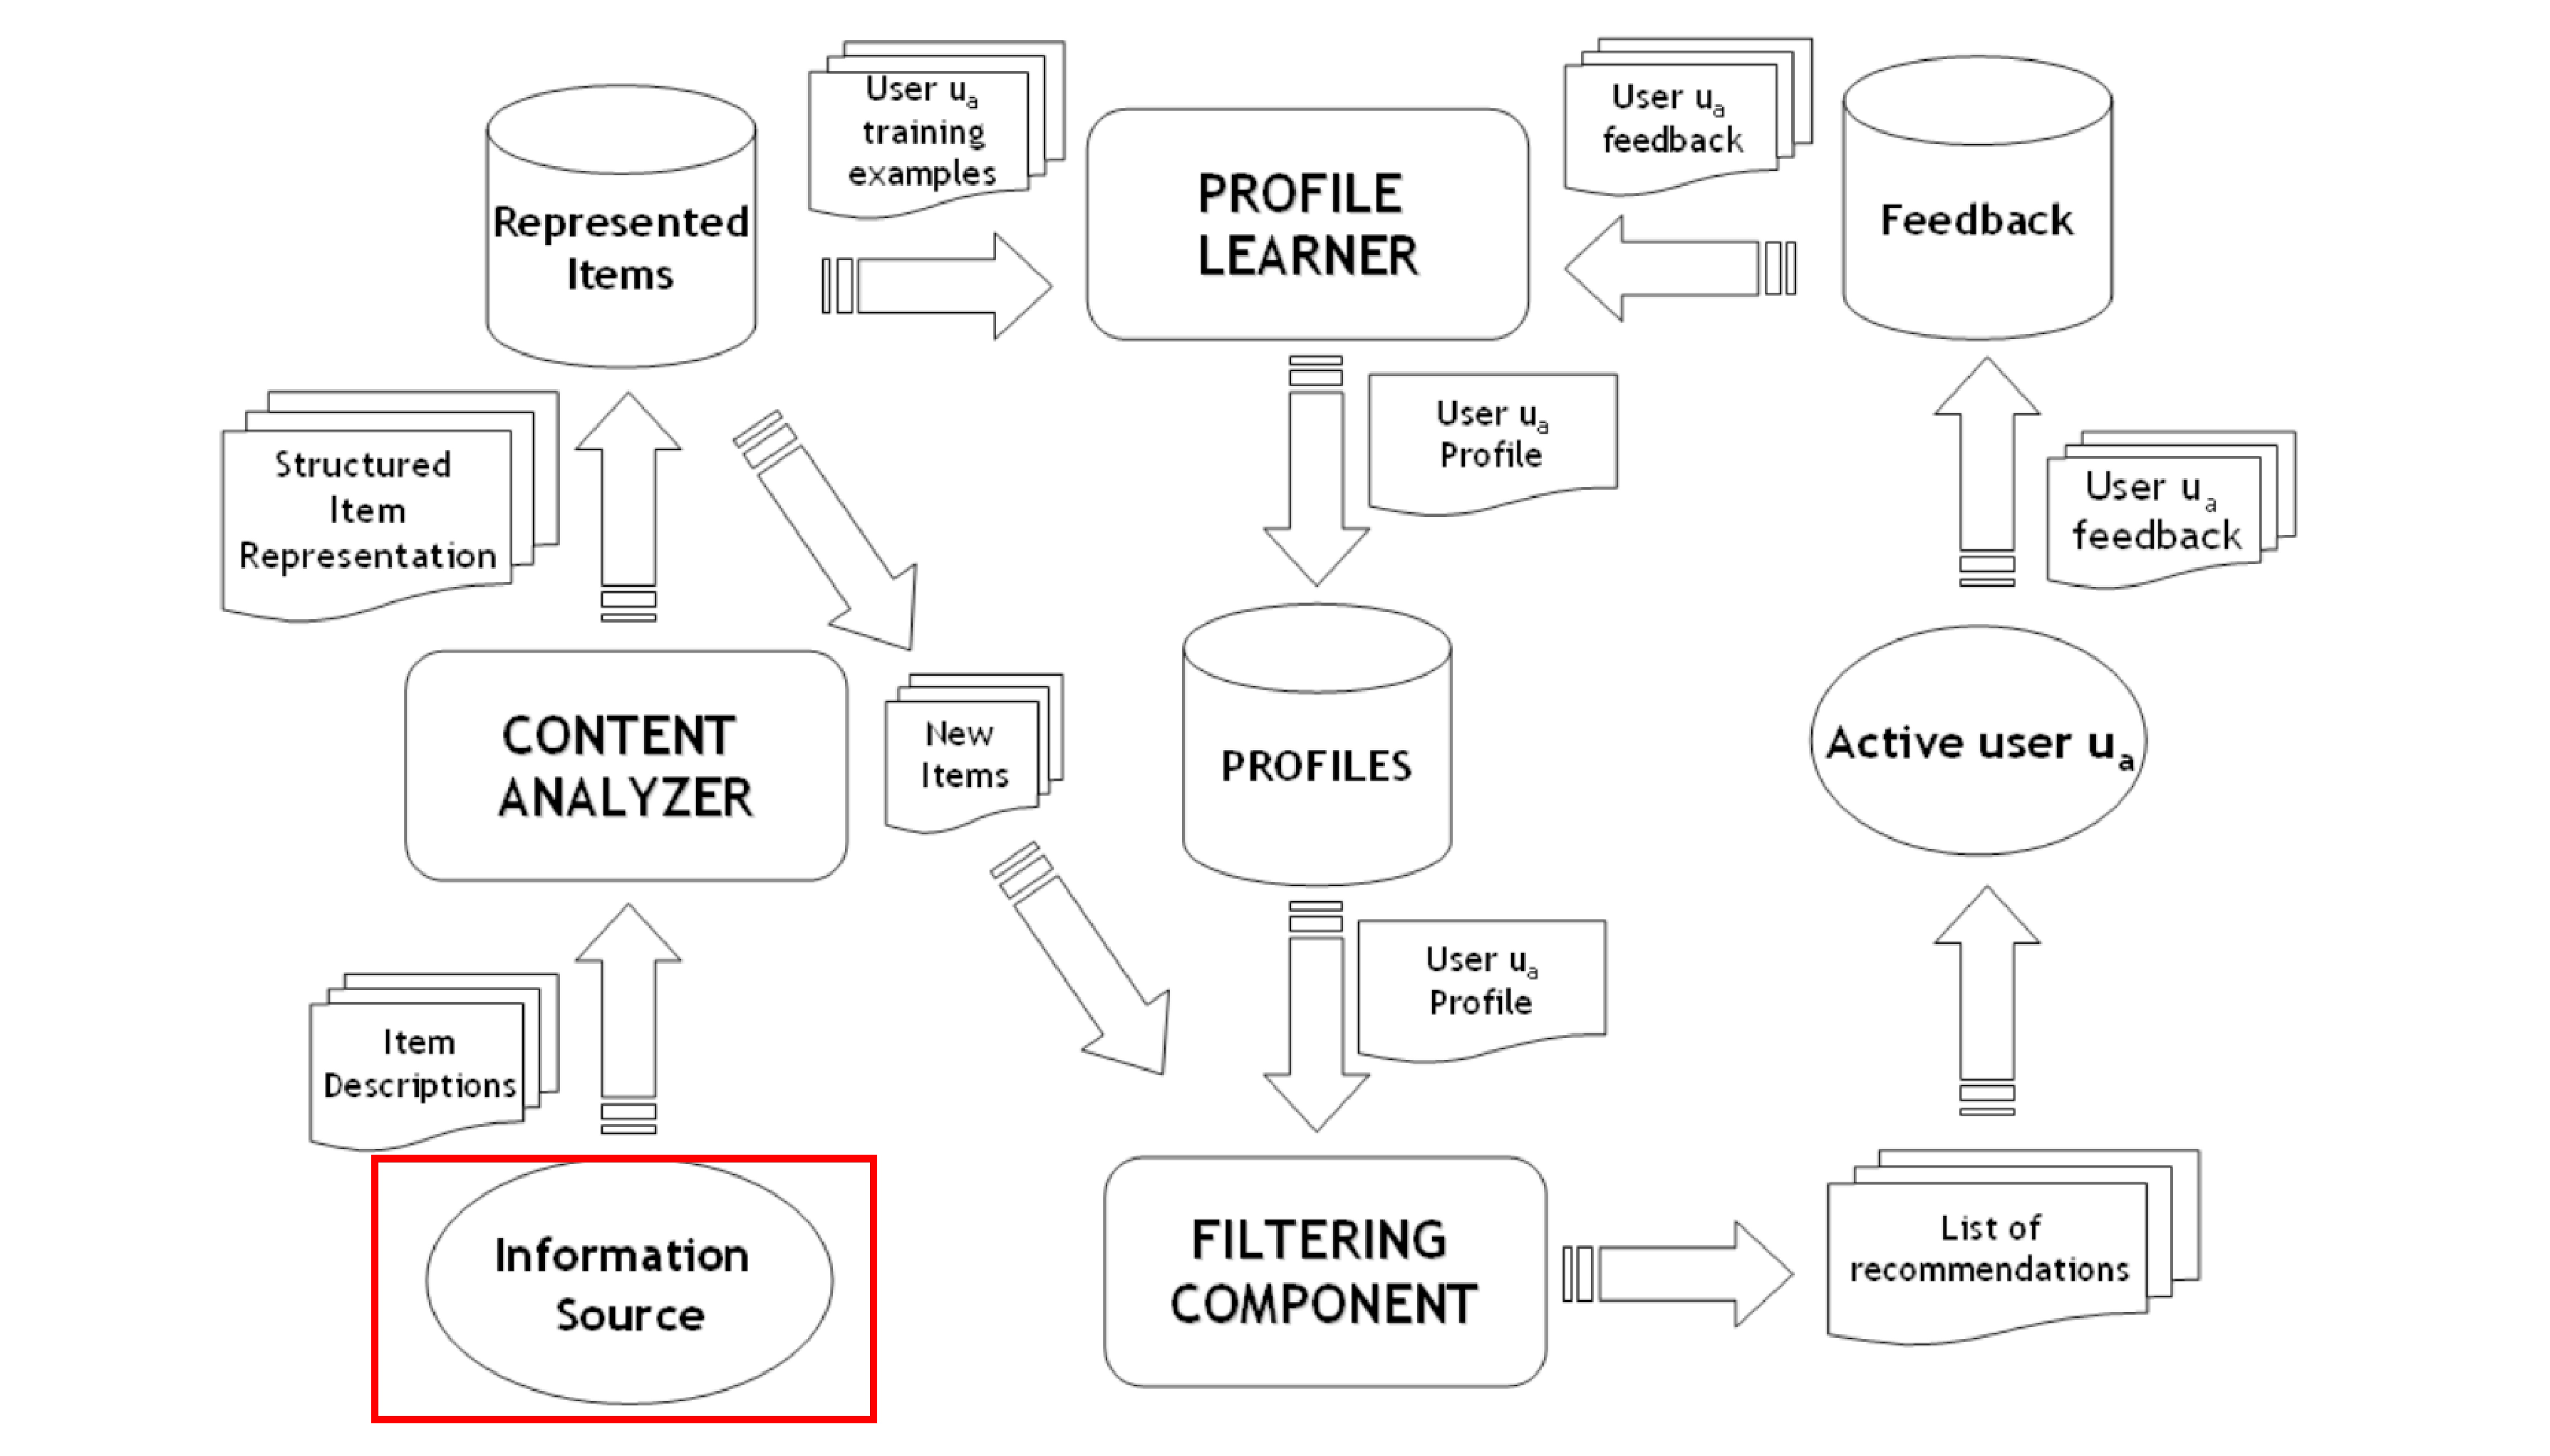
\includegraphics[width=1\textwidth]{figura/recomendacao_conteudo_1.eps}
  \caption{Fluxo para construção de um sistema de recomendação por conteúdo (LOPS; GEMMIS; SEMERARO, 2011)}
\end{figure}

\end{frame}

\begin{frame}

\begin{figure}[h!]
  \centering
    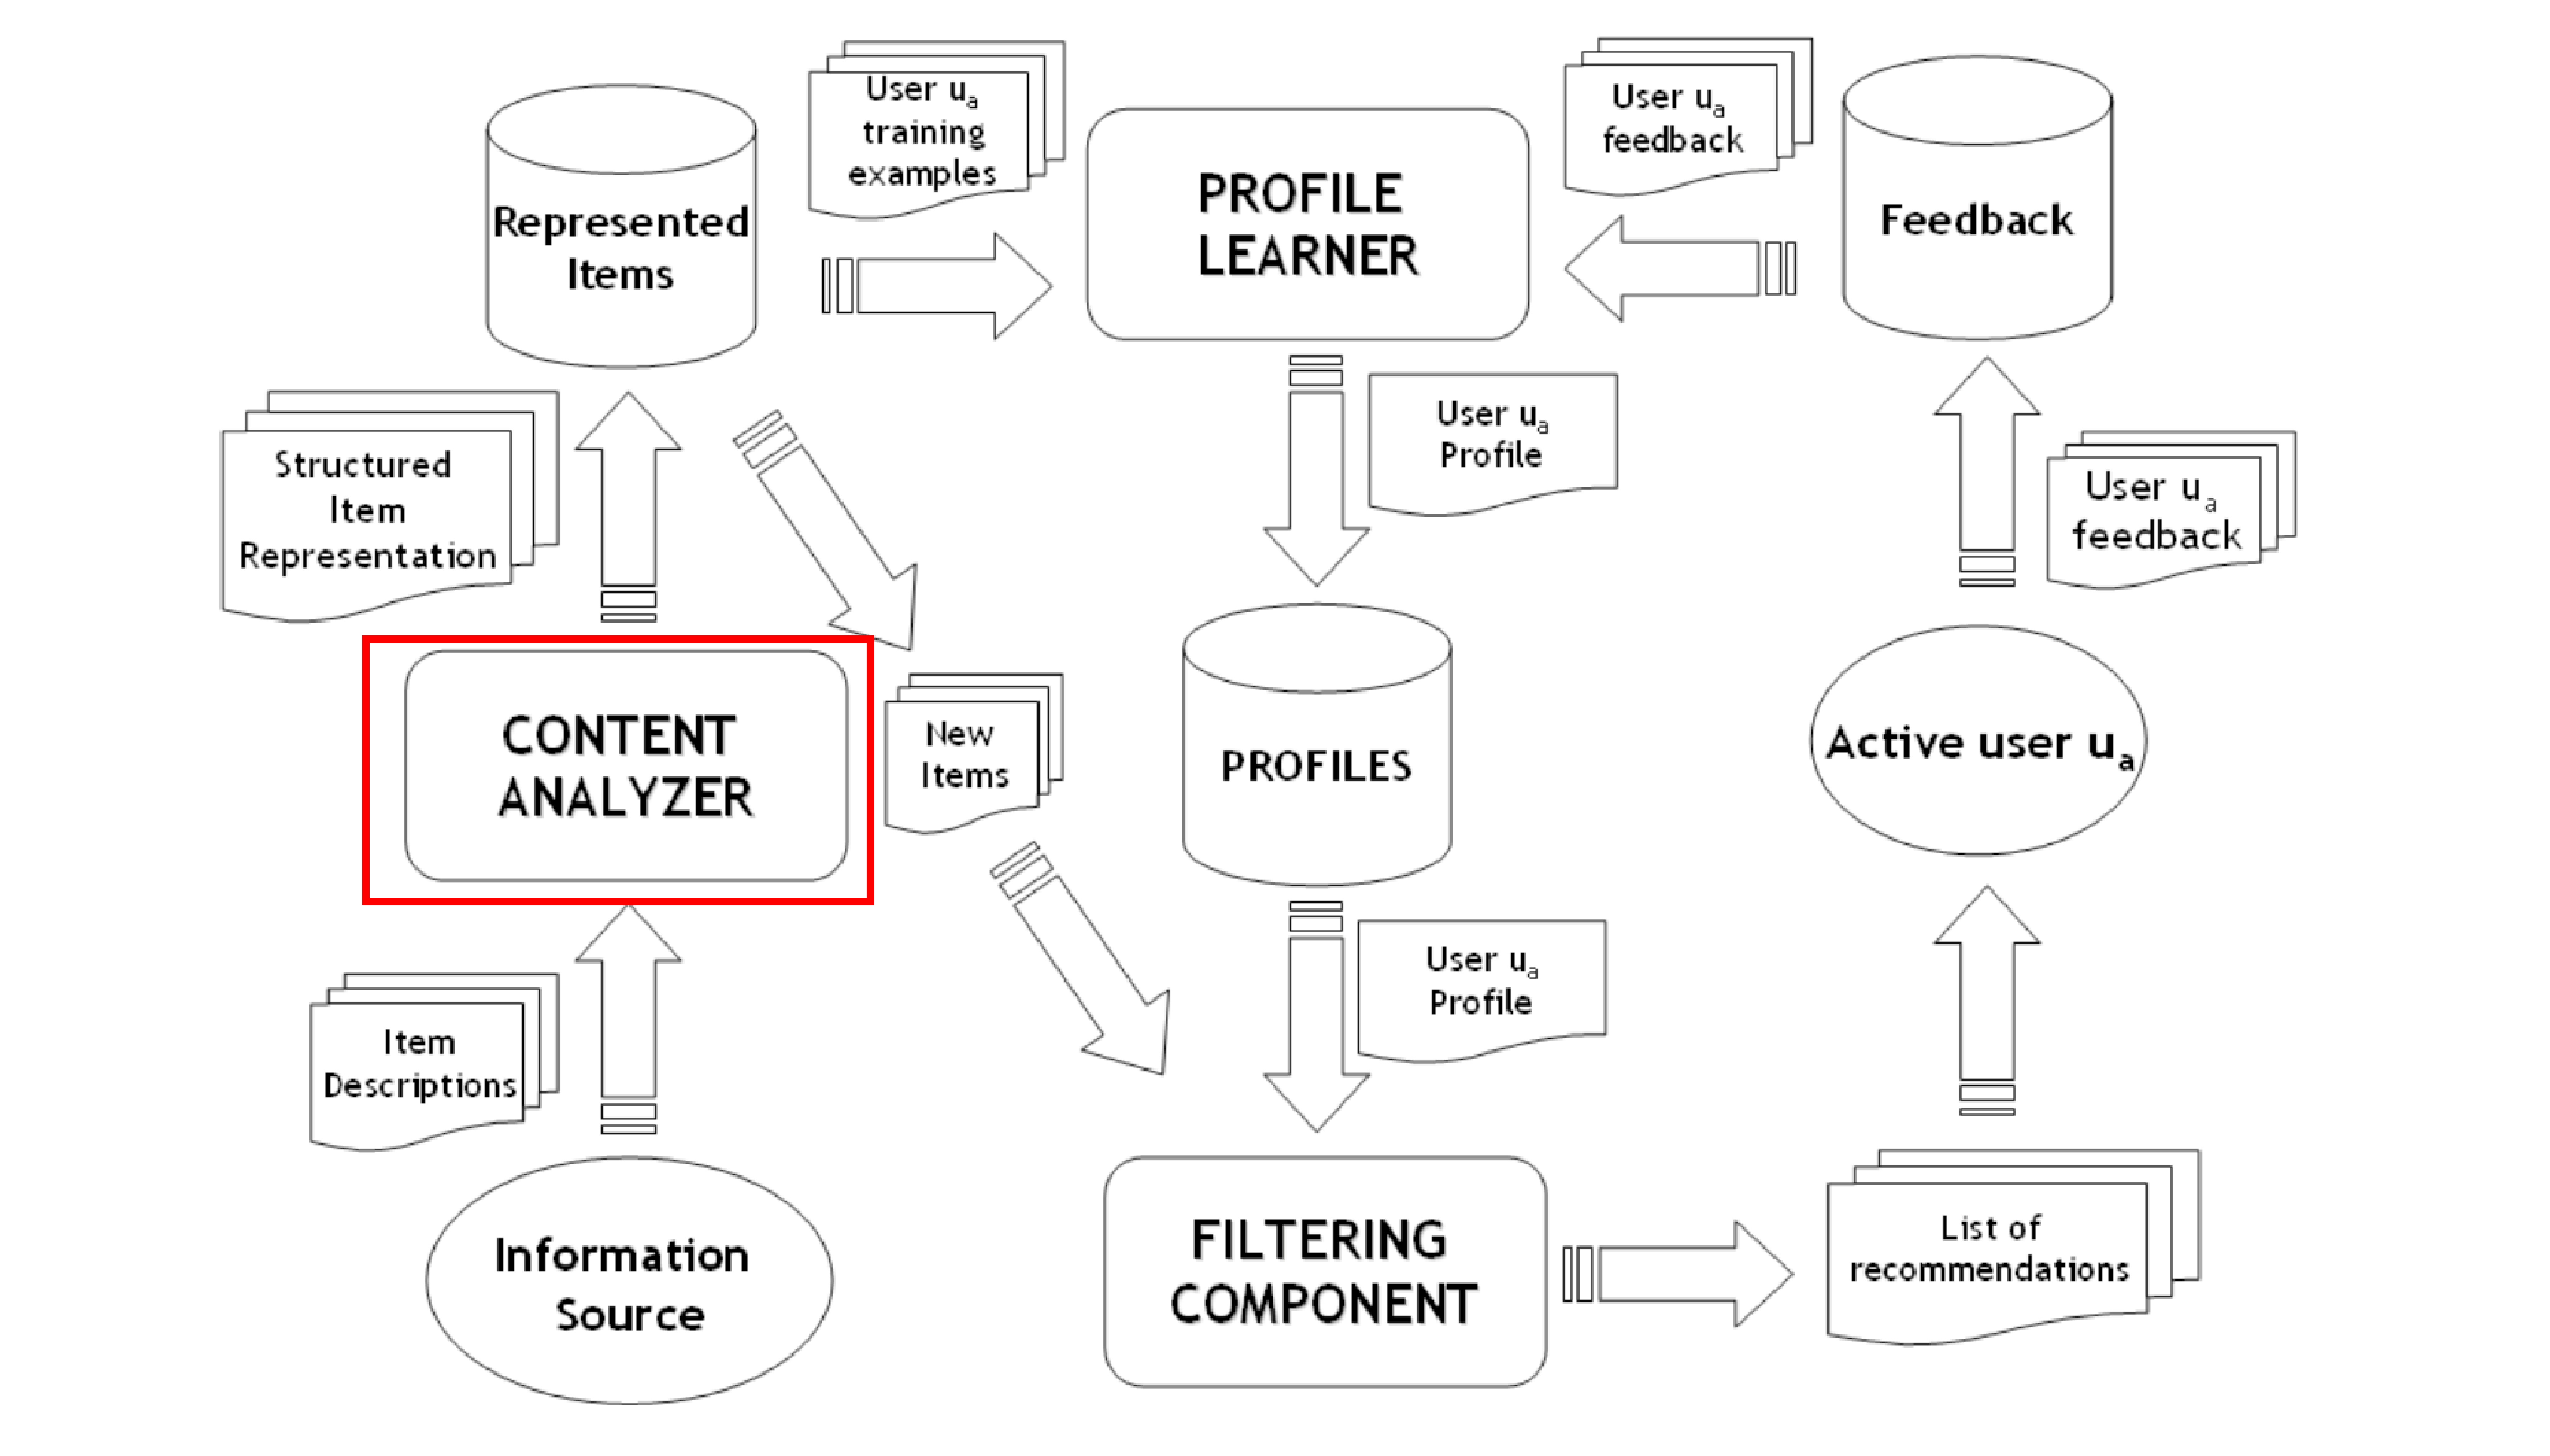
\includegraphics[width=1\textwidth]{figura/recomendacao_conteudo_2.eps}
  \caption{Fluxo para construção de um sistema de recomendação por conteúdo (LOPS; GEMMIS; SEMERARO, 2011)}
\end{figure}

\end{frame}

\begin{frame}

\begin{figure}[h!]
  \centering
    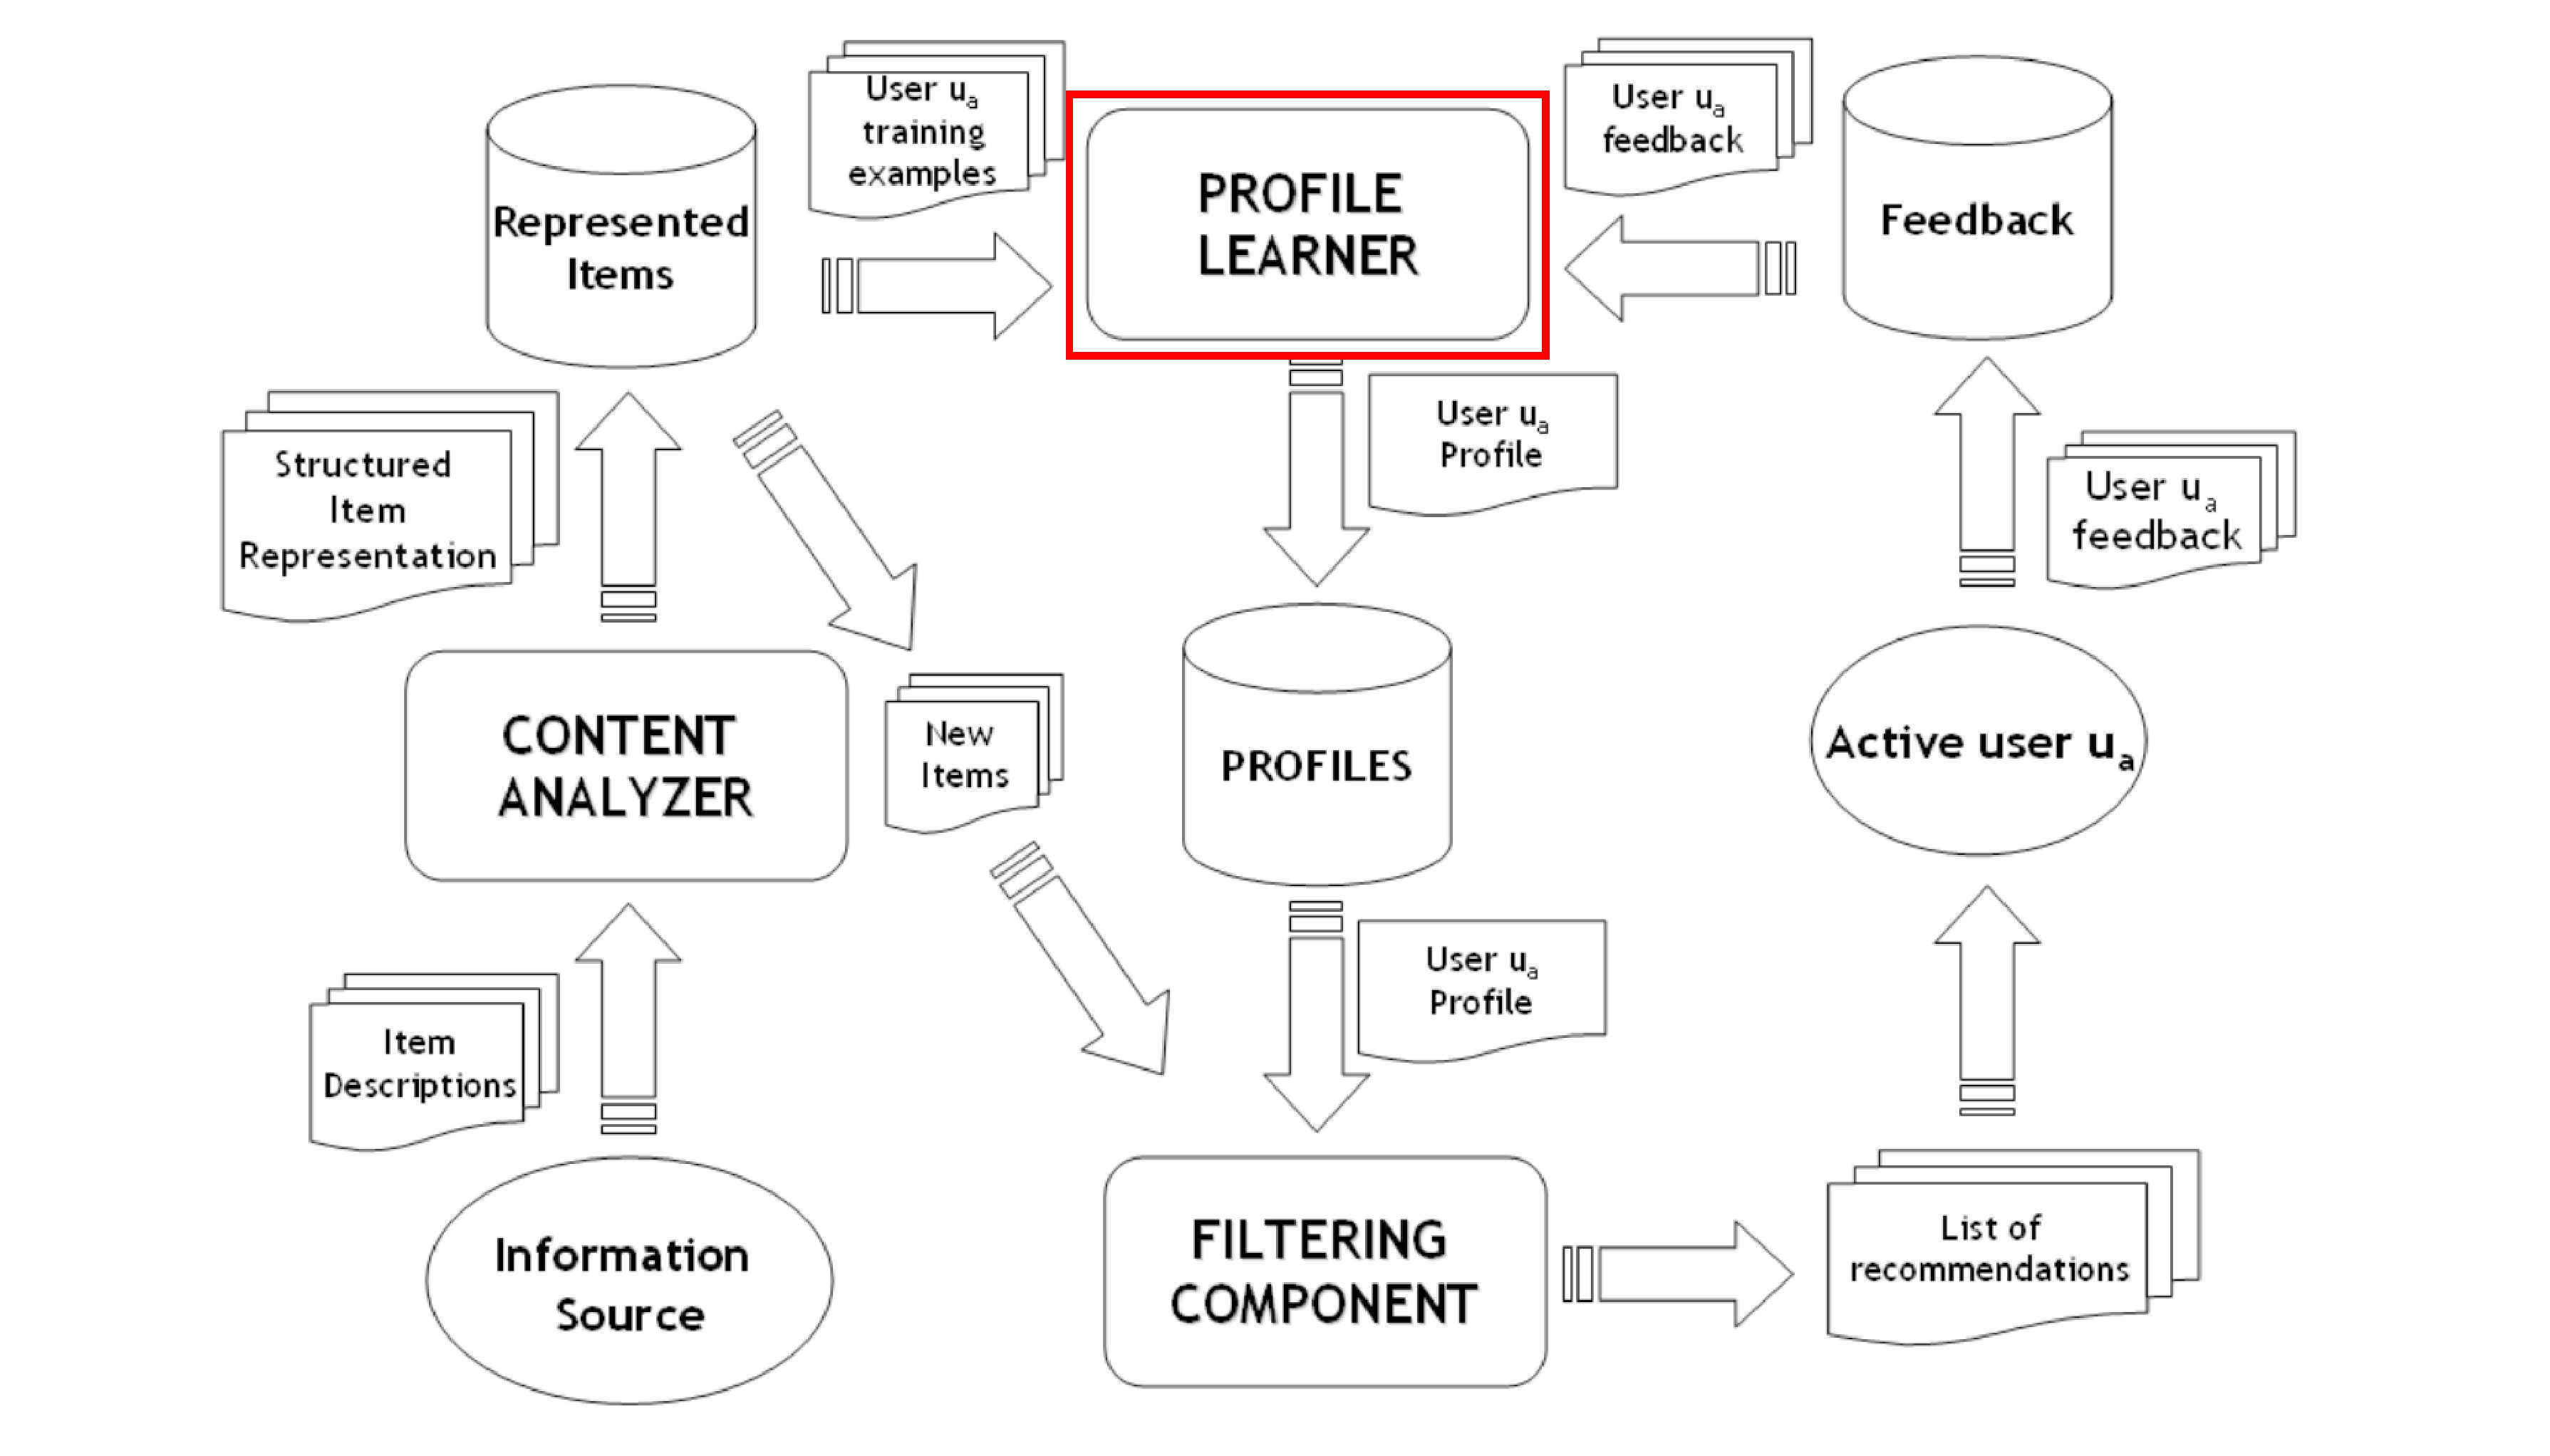
\includegraphics[width=1\textwidth]{figura/recomendacao_conteudo_3.eps}
  \caption{Fluxo para construção de um sistema de recomendação por conteúdo (LOPS; GEMMIS; SEMERARO, 2011)}
\end{figure}

\end{frame}

\begin{frame}

\begin{figure}[h!]
  \centering
    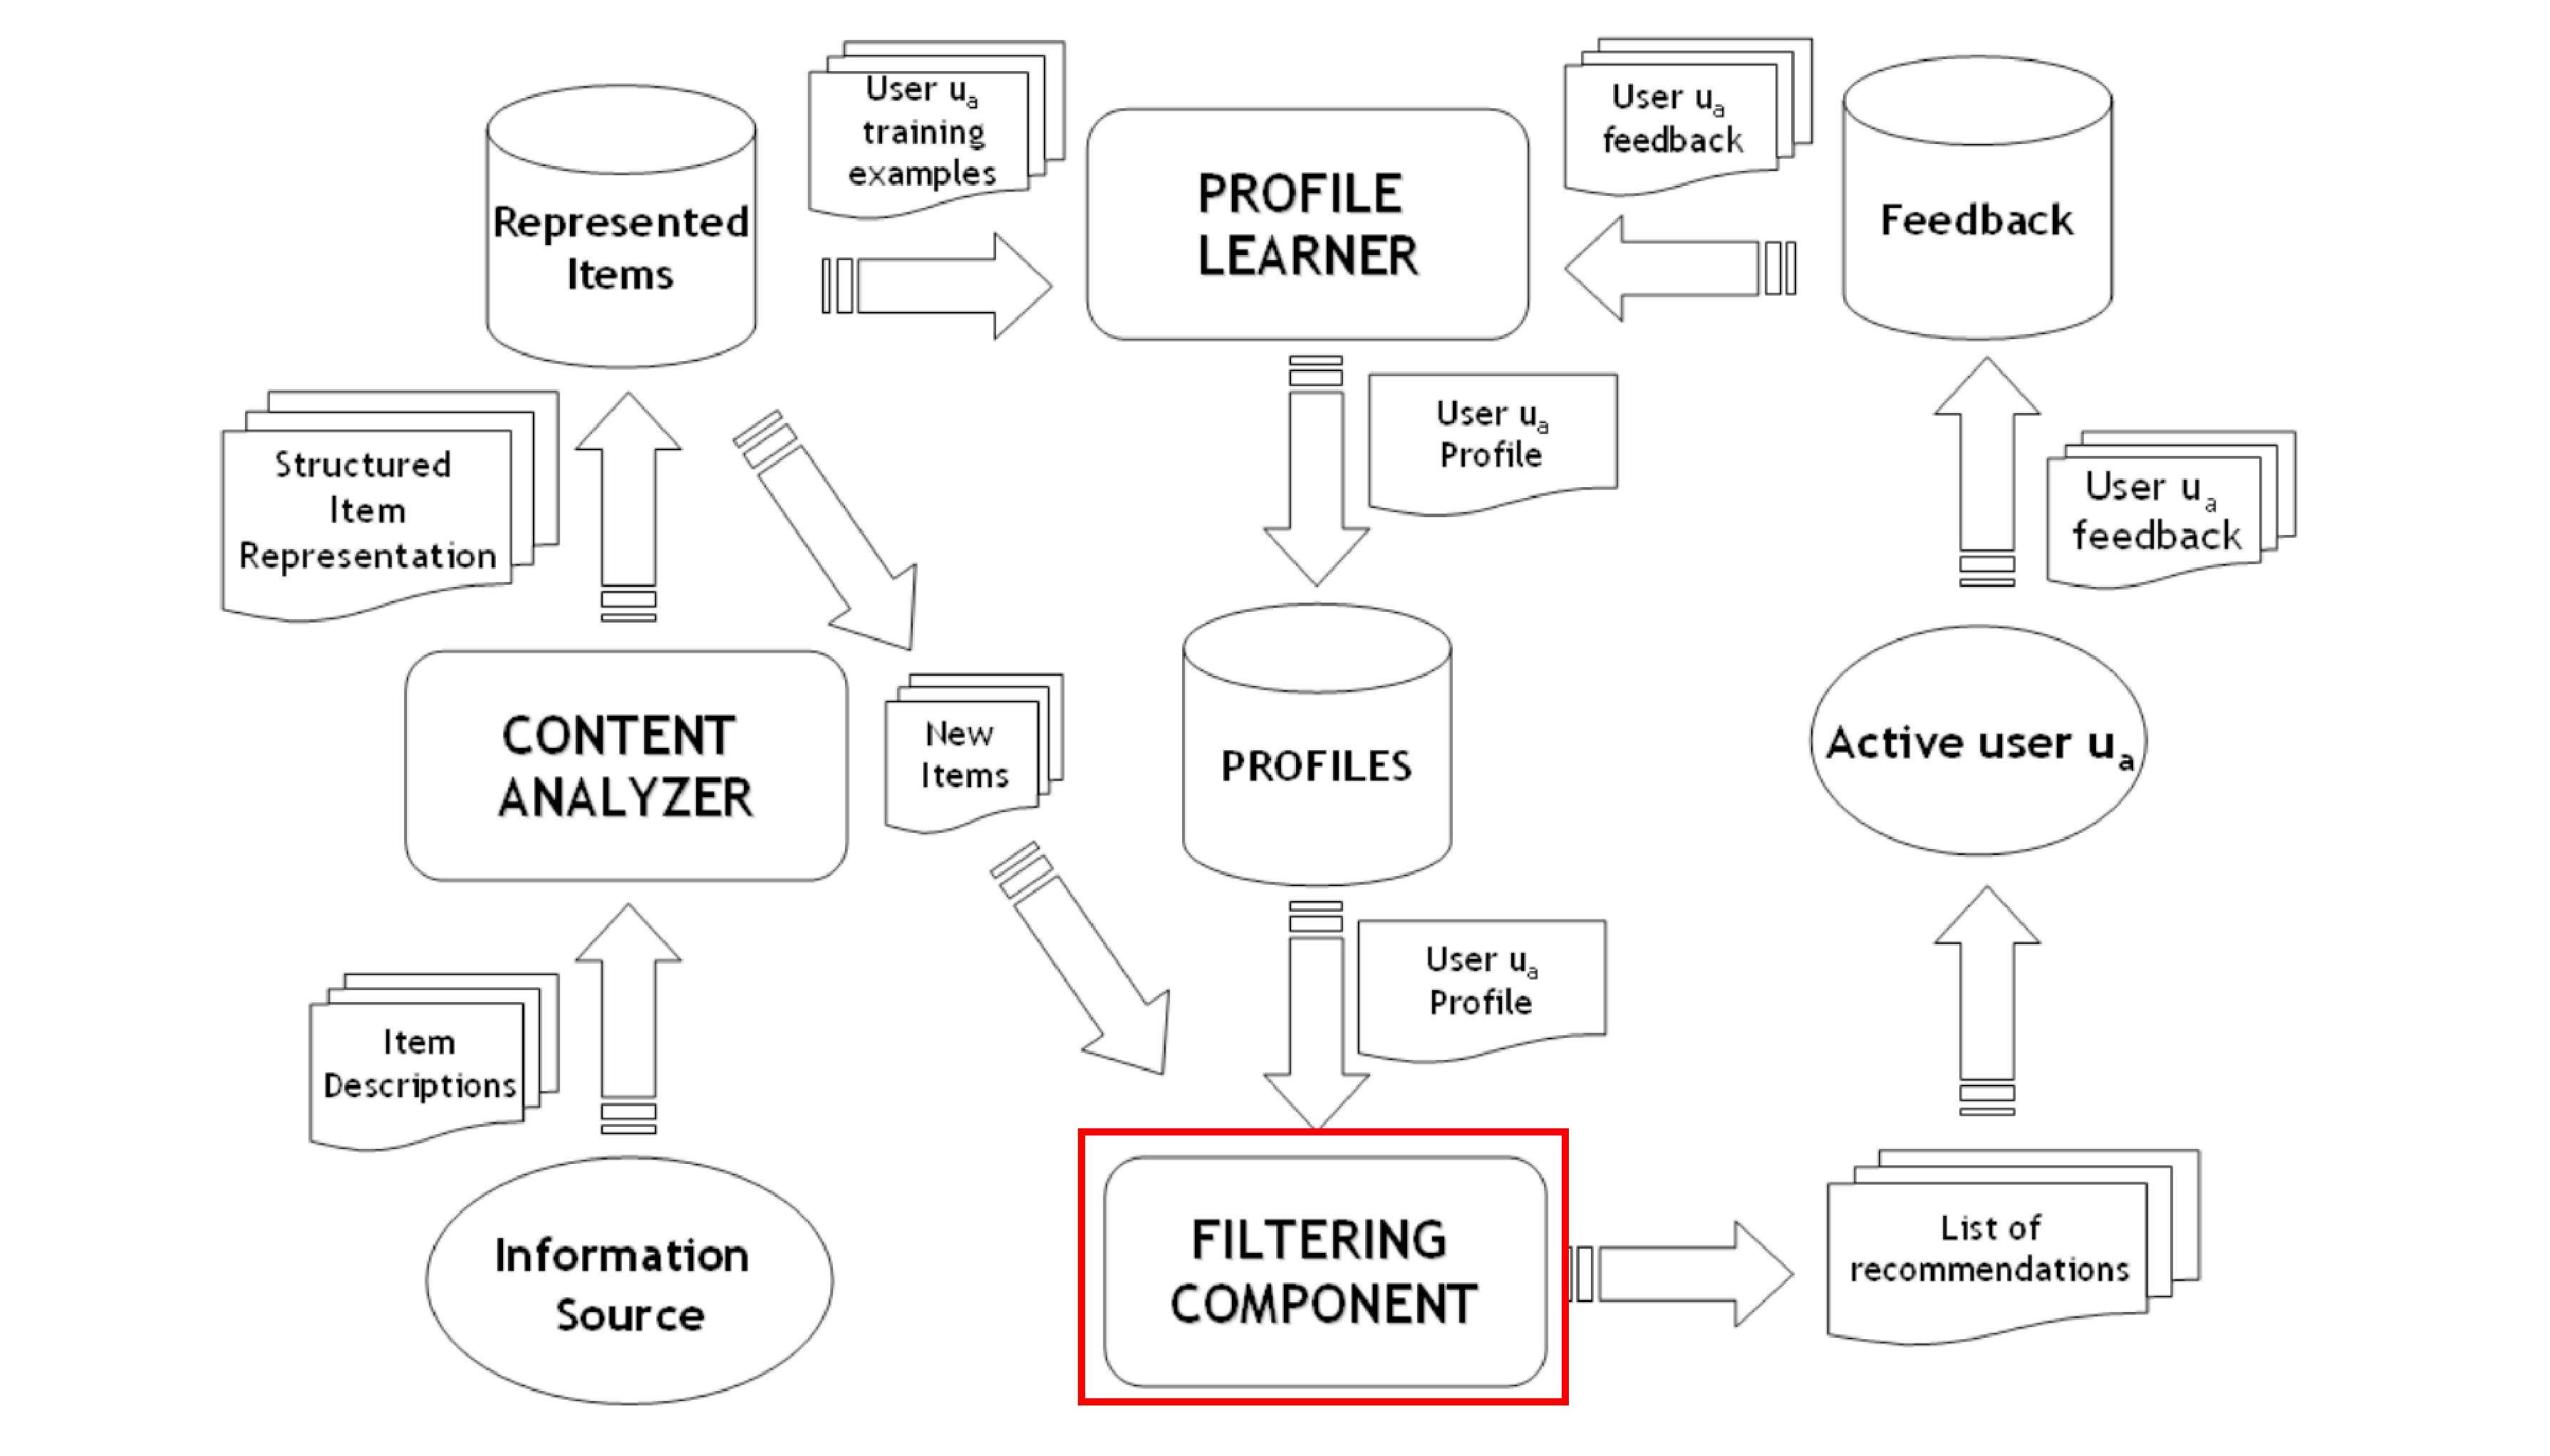
\includegraphics[width=1\textwidth]{figura/recomendacao_conteudo_4.eps}
  \caption{Fluxo para construção de um sistema de recomendação por conteúdo (LOPS; GEMMIS; SEMERARO, 2011)}
\end{figure}

\end{frame}

\begin{frame}

\begin{figure}[h!]
  \centering
    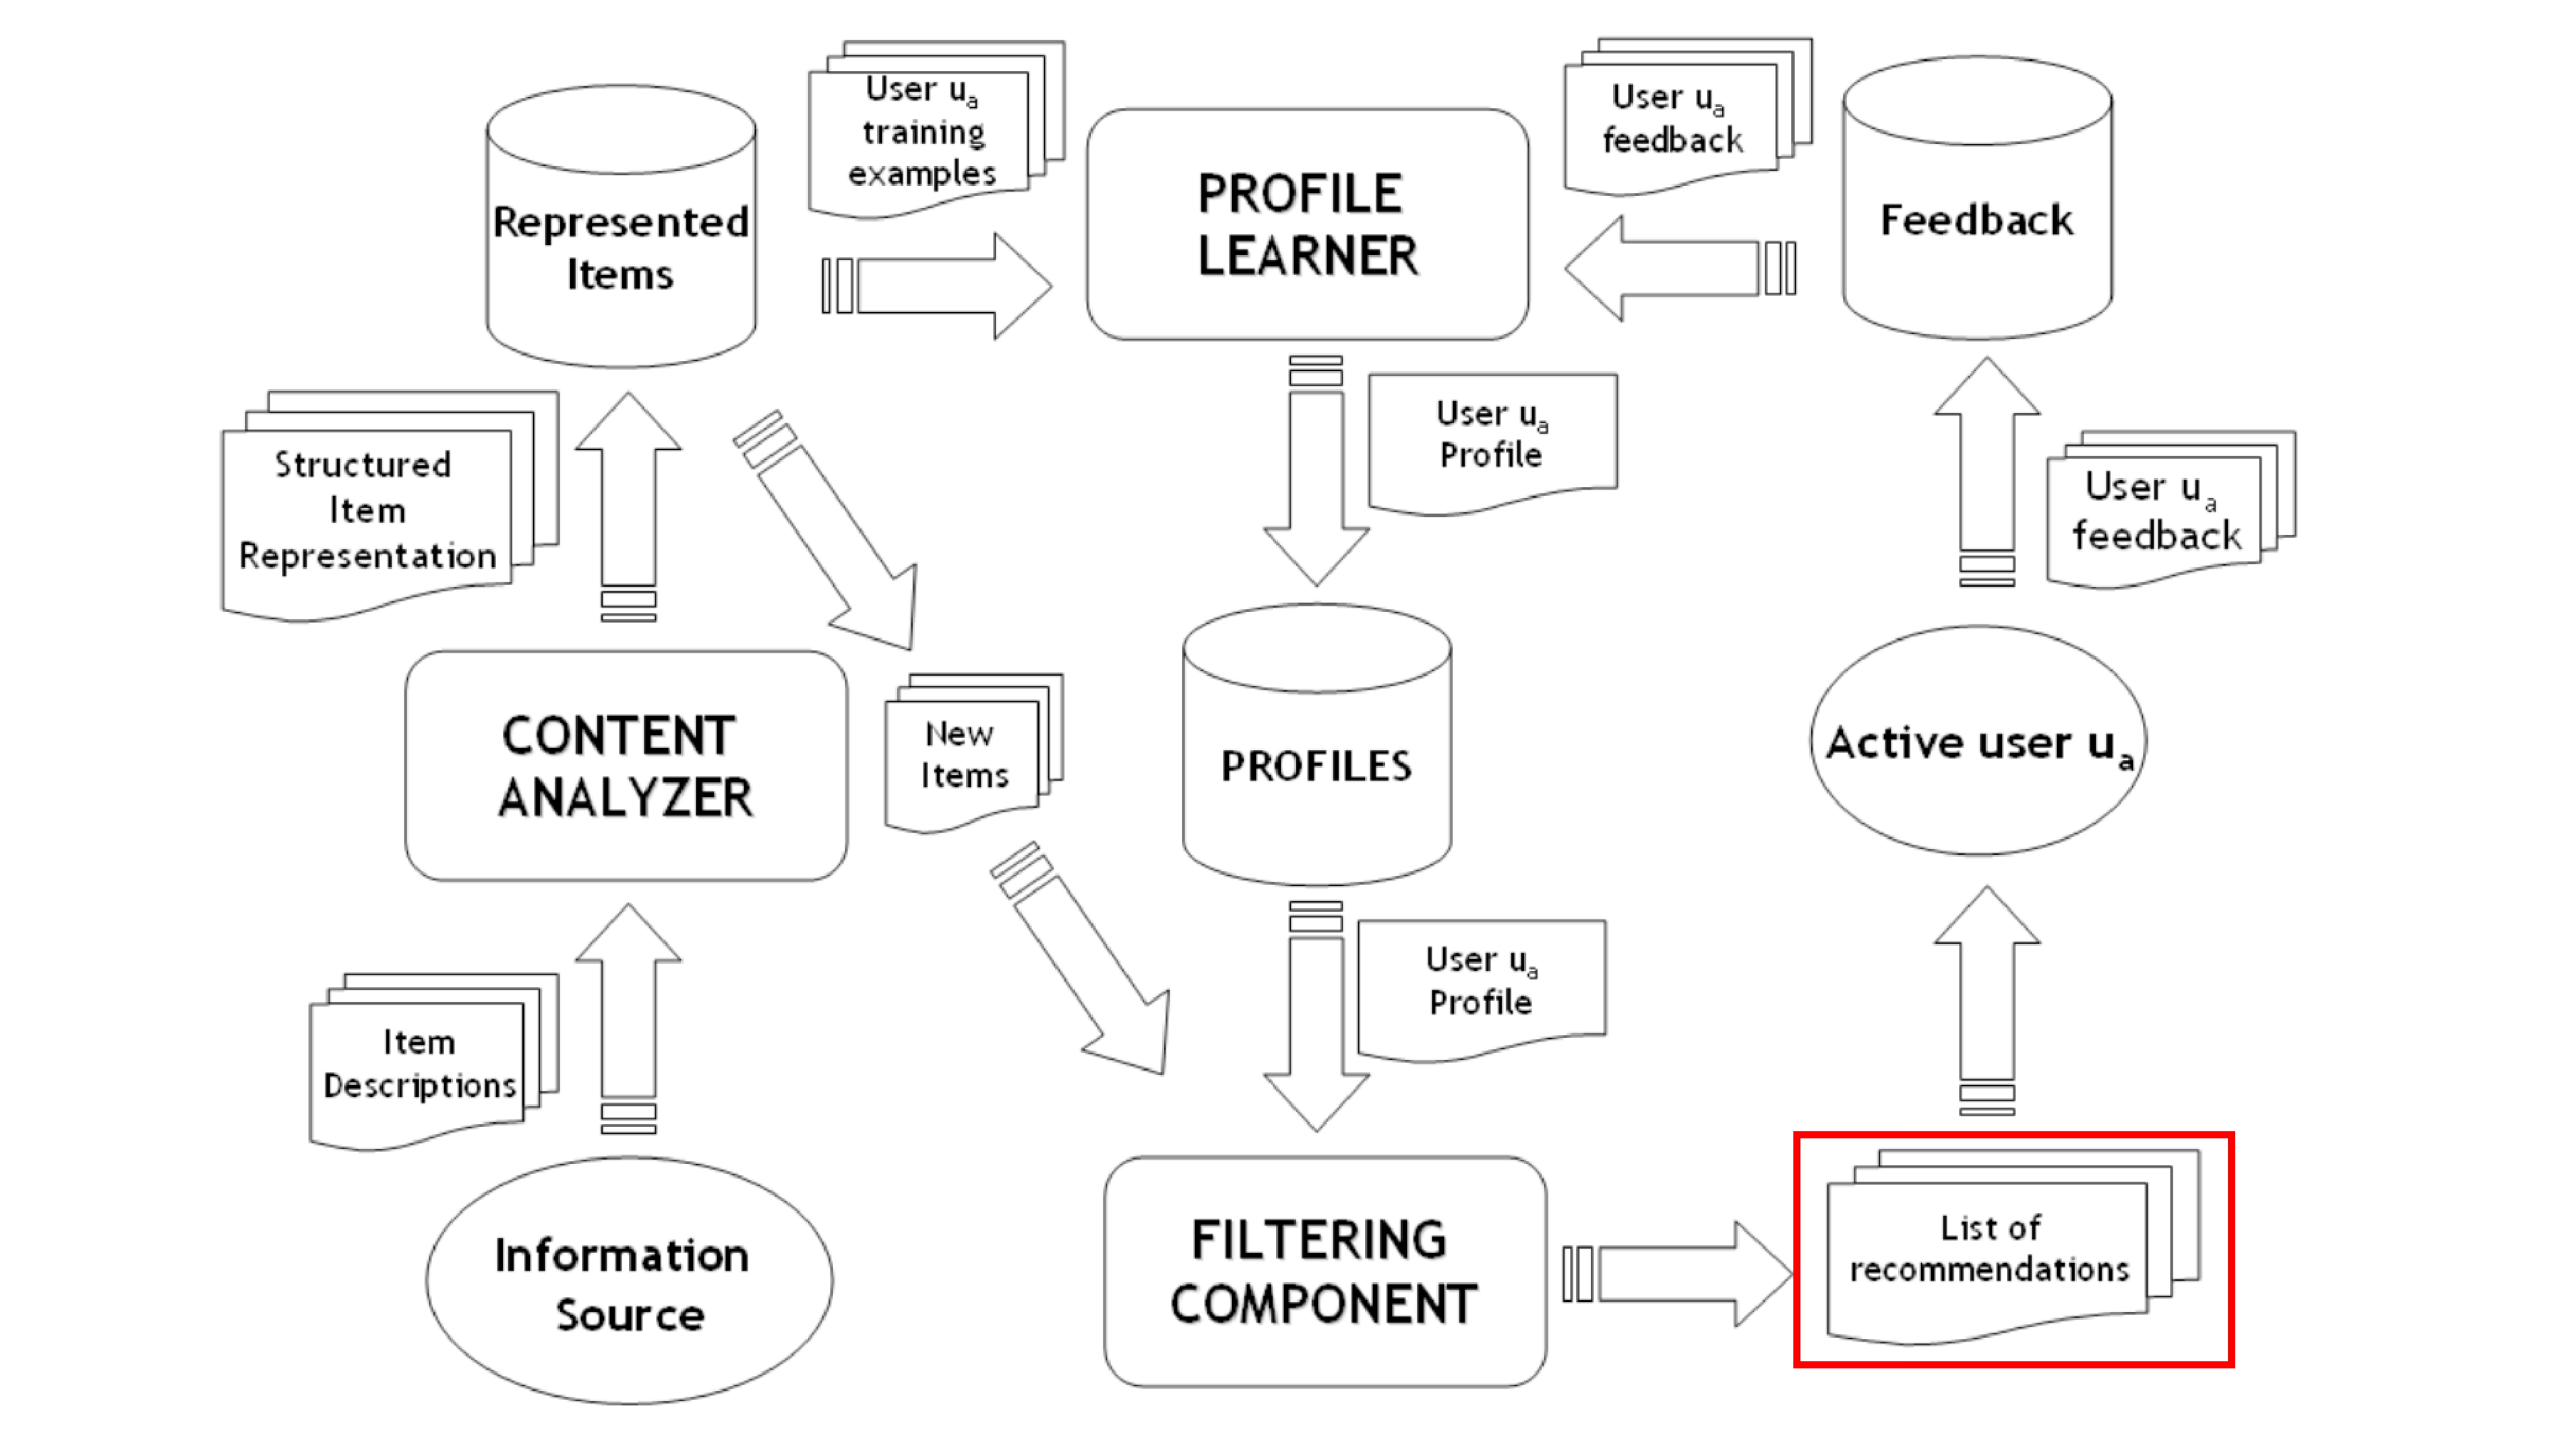
\includegraphics[width=1\textwidth]{figura/recomendacao_conteudo_5.eps}
  \caption{Fluxo para construção de um sistema de recomendação por conteúdo (LOPS; GEMMIS; SEMERARO, 2011)}
\end{figure}

\end{frame}

\begin{frame}

\begin{figure}[h!]
  \centering
    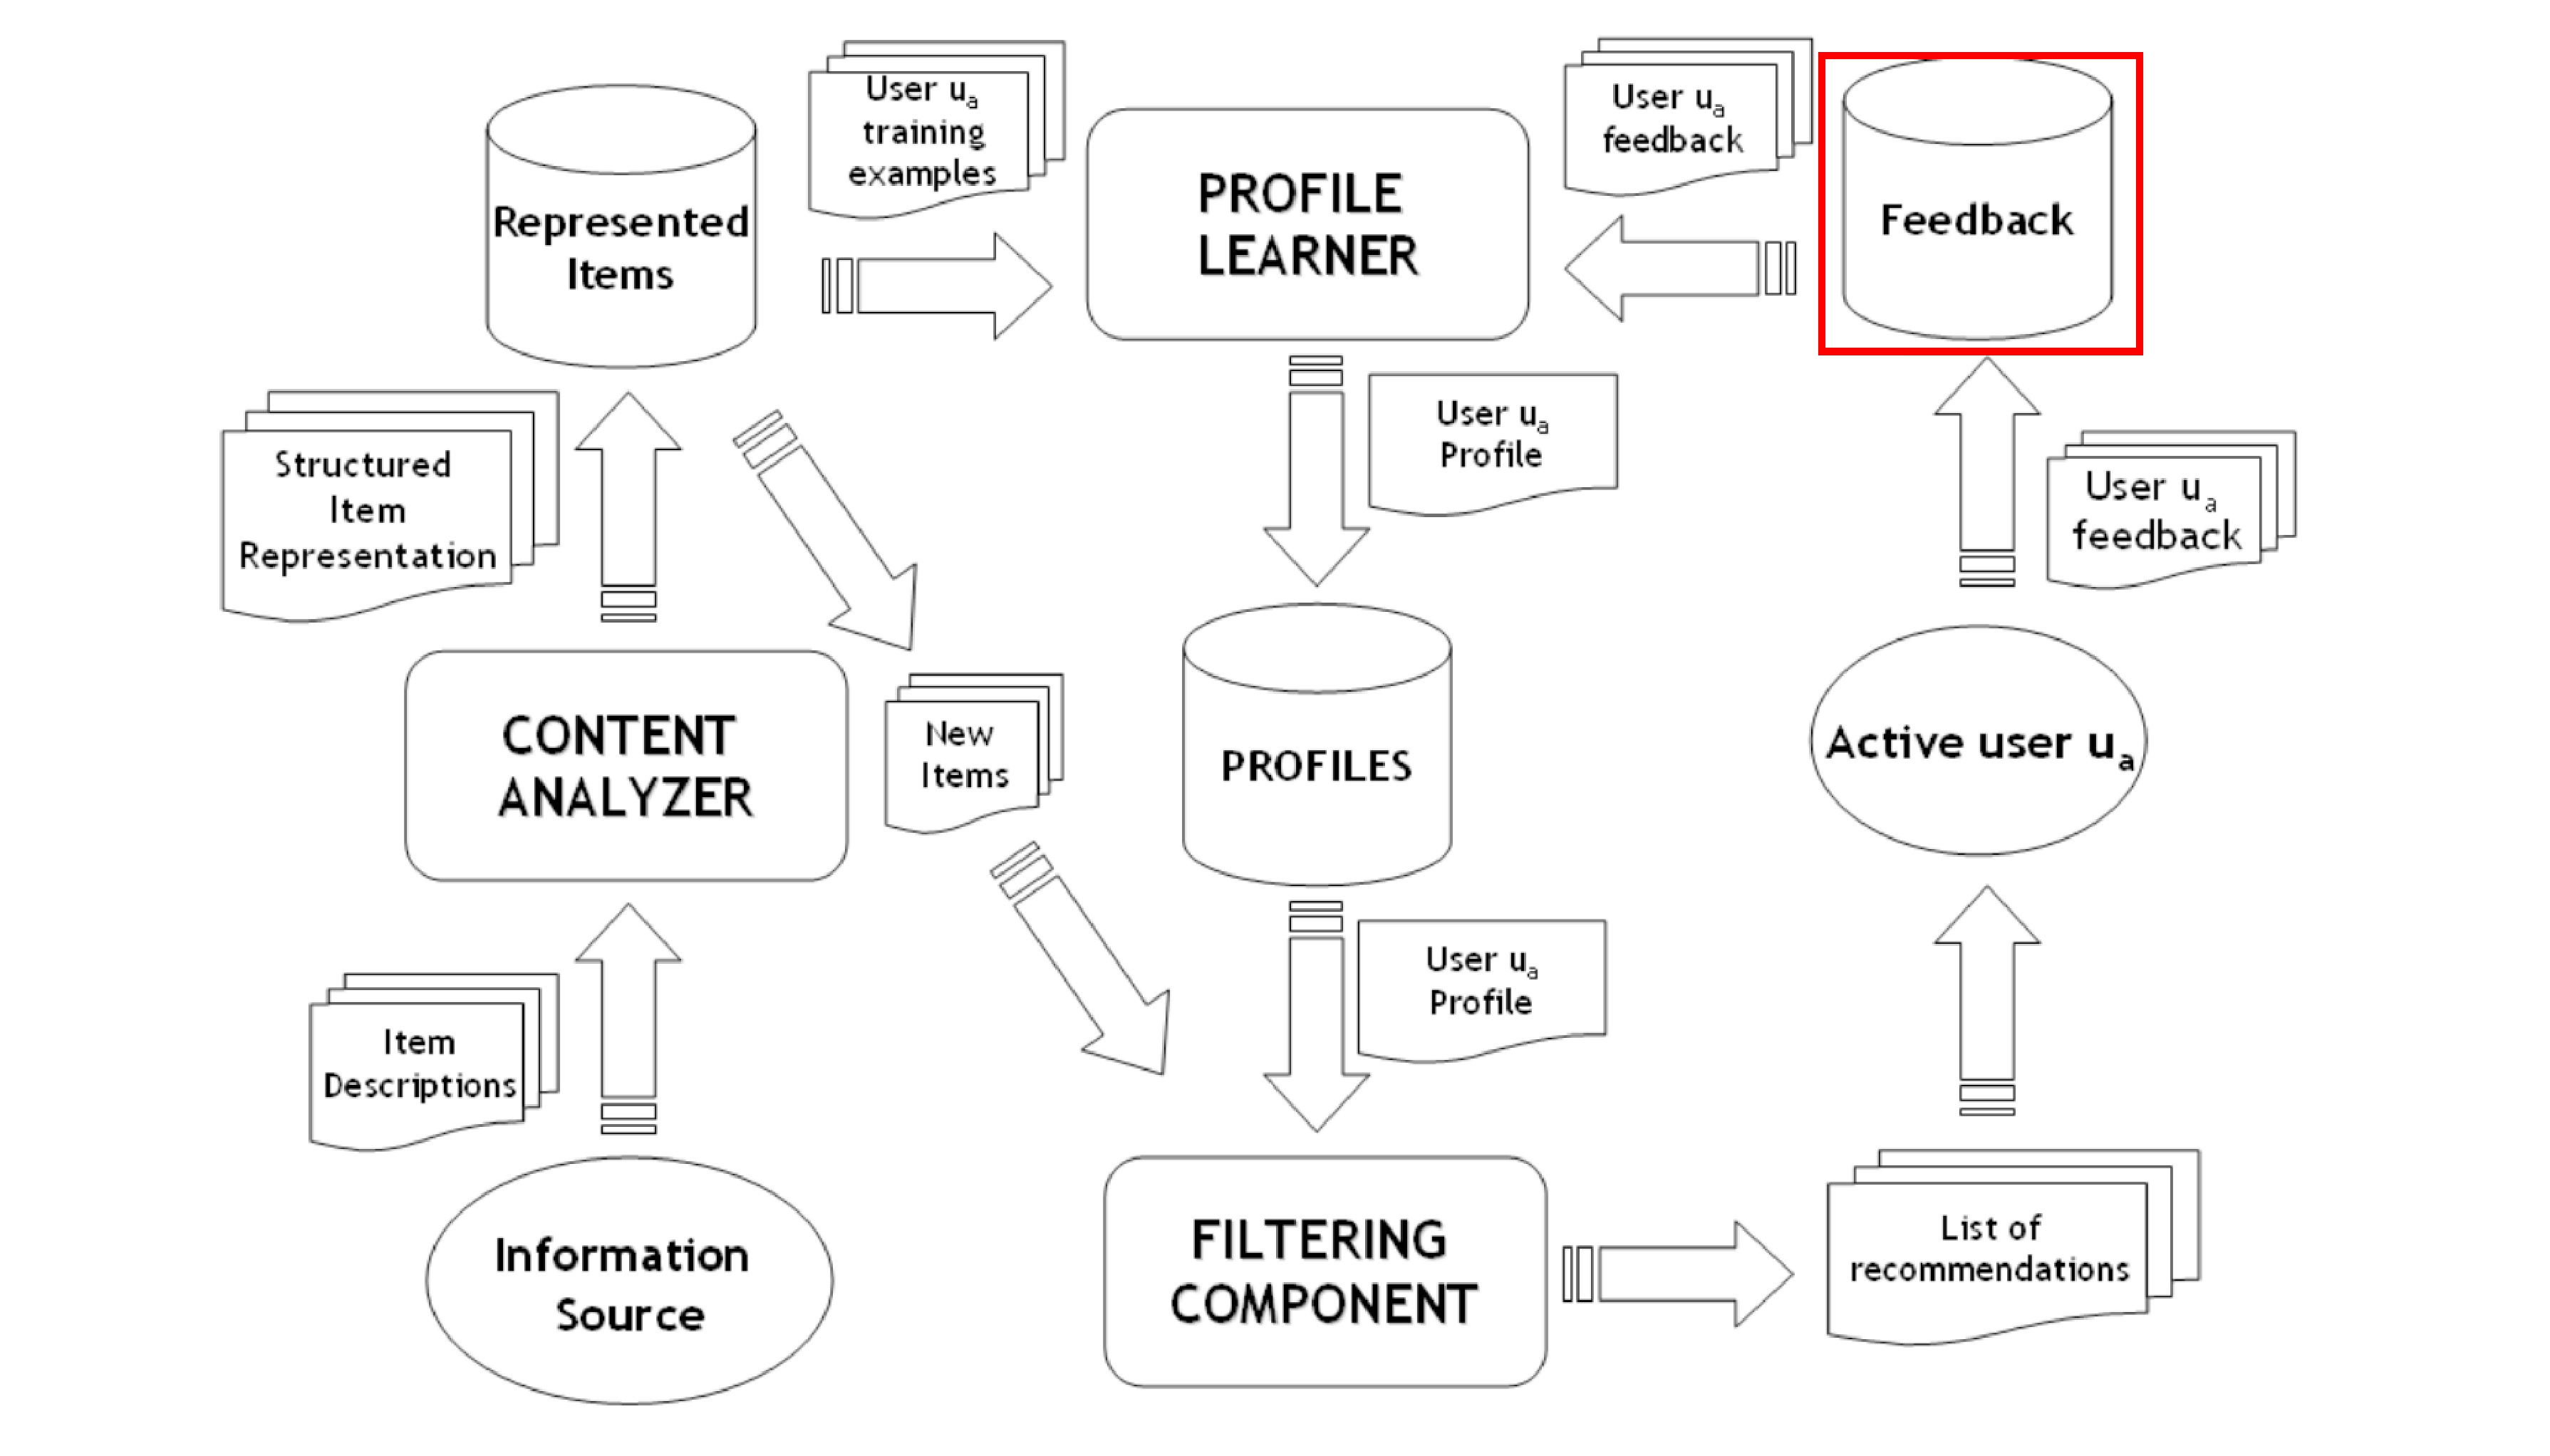
\includegraphics[width=1\textwidth]{figura/recomendacao_conteudo_6.eps}
  \caption{Fluxo para construção de um sistema de recomendação por conteúdo (LOPS; GEMMIS; SEMERARO, 2011)}
\end{figure}

\end{frame}


% section l (end)

\section{Software escolhido} % (fold)
\label{sec:software_escolhido}
\begin{frame}
\begin{itemize}
    \item AppRecommender

    \item \say{\textit{dada a lista de programas instalados em determinado sistema,
          o recomendador retorna uma lista de aplicativos sugeridos, que supostamente
          são aplicativos de potencial interesse para os usuários daquele sistema}}, \\ARAÚJO, T. C
\end{itemize}
\end{frame}

\begin{frame}
\begin{figure}[h]
  \centering
  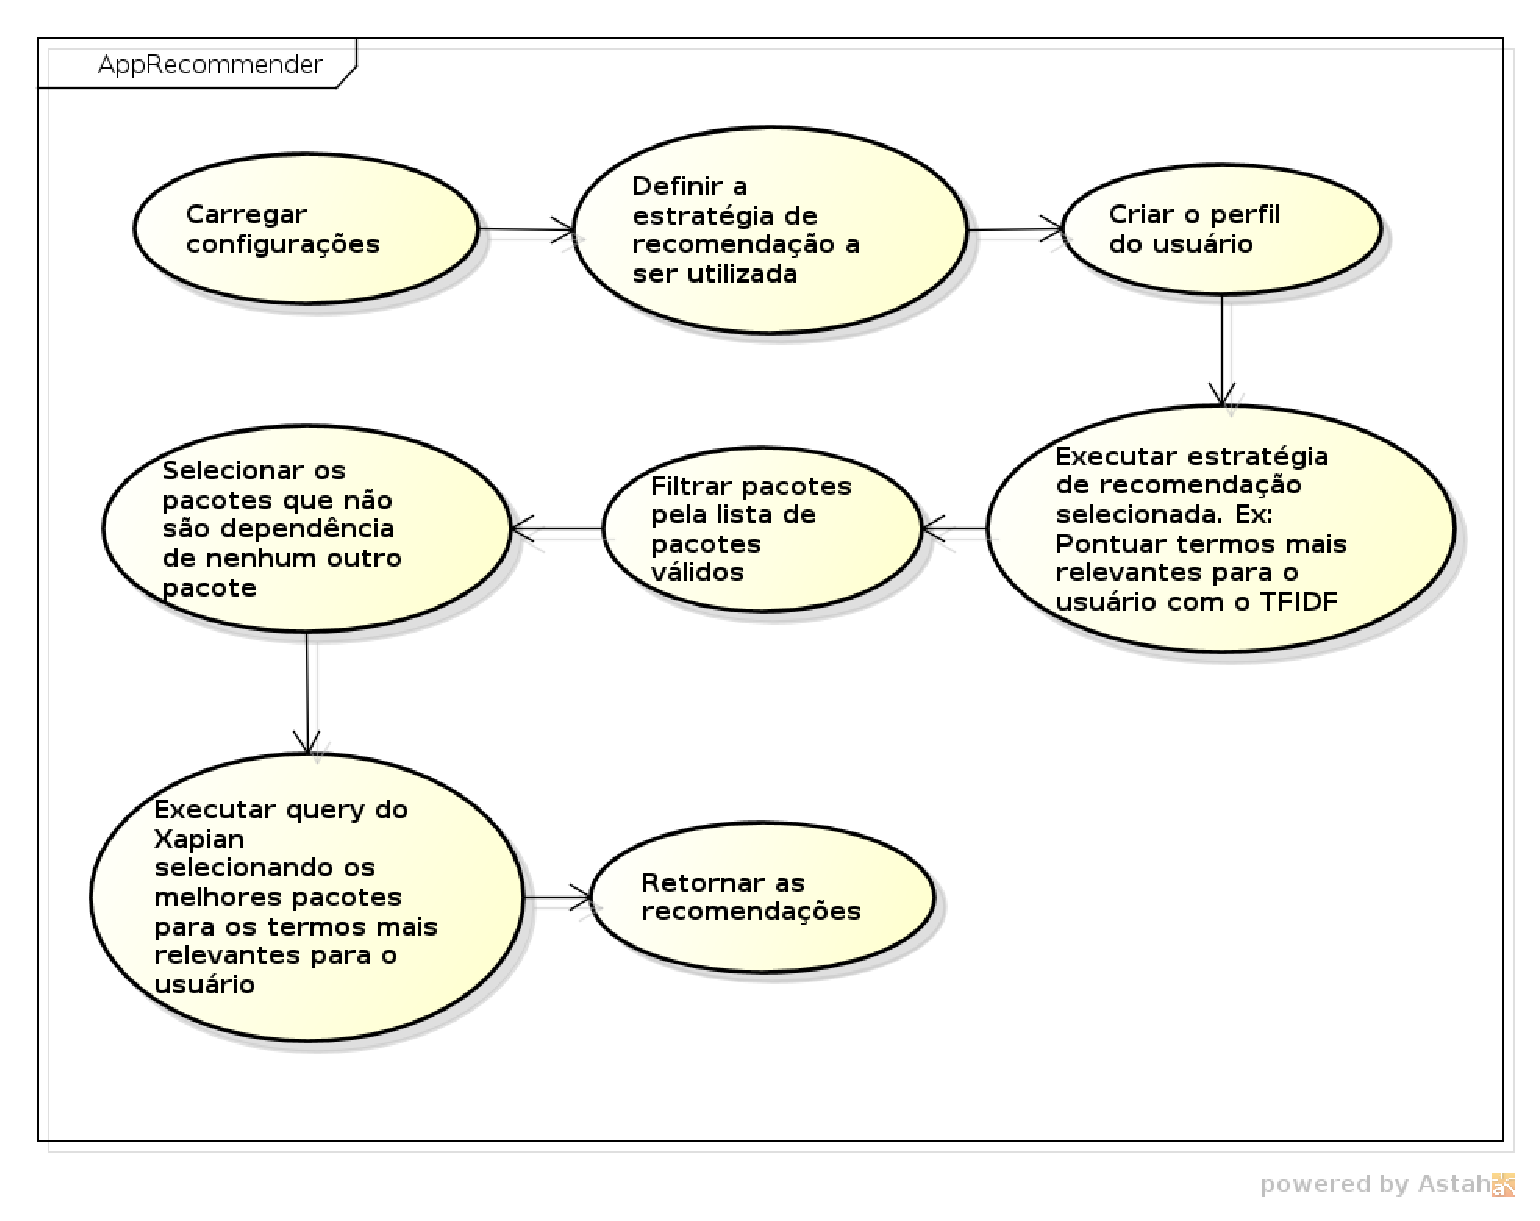
\includegraphics[width=0.9\textwidth]{figura/app_recommender_process.eps}
  \caption{Processo do AppRecommender}
  \label{fig:curva_aprendizado}
\end{figure}
\end{frame}

\begin{frame}
    Perfil de Usuário
    \begin{itemize}
        \item Lista de termos mais significativos para o usuário
        \item Uma estratégia de recomendação é responsável por definir quais termos
        são usados no perfil do usuário
    \end{itemize}

    \begin{table}[h]
    \centering
    \begin{tabular}{cc}
    \hline
    \rowcolor[HTML]{EFEFEF}
    {Termos} & {Perfil do usuário} \\ \hline
    {devel::editor} & {devel::editor} \\ \hline
    {implemented-in::c} & {role::program} \\ \hline
    {role::program} & {} \\ \hline
    {interface::commandline} & {} \\ \hline
    {interface::text-mode} & {} \\ \hline
    \end{tabular}
    \caption{Exemplo de termos e perfil do usuário}
    \label{tab:classificacao_pacotes}
    \end{table}
\end{frame}

\section{Contexto temporal no Debian} % (fold)
\label{sec:d}

\begin{frame}

    \begin{itemize}
        \item Stat
        \item Popularity-contest
    \end{itemize}

\end{frame}

\begin{frame}
\begin{figure}[h!]
    \centering
    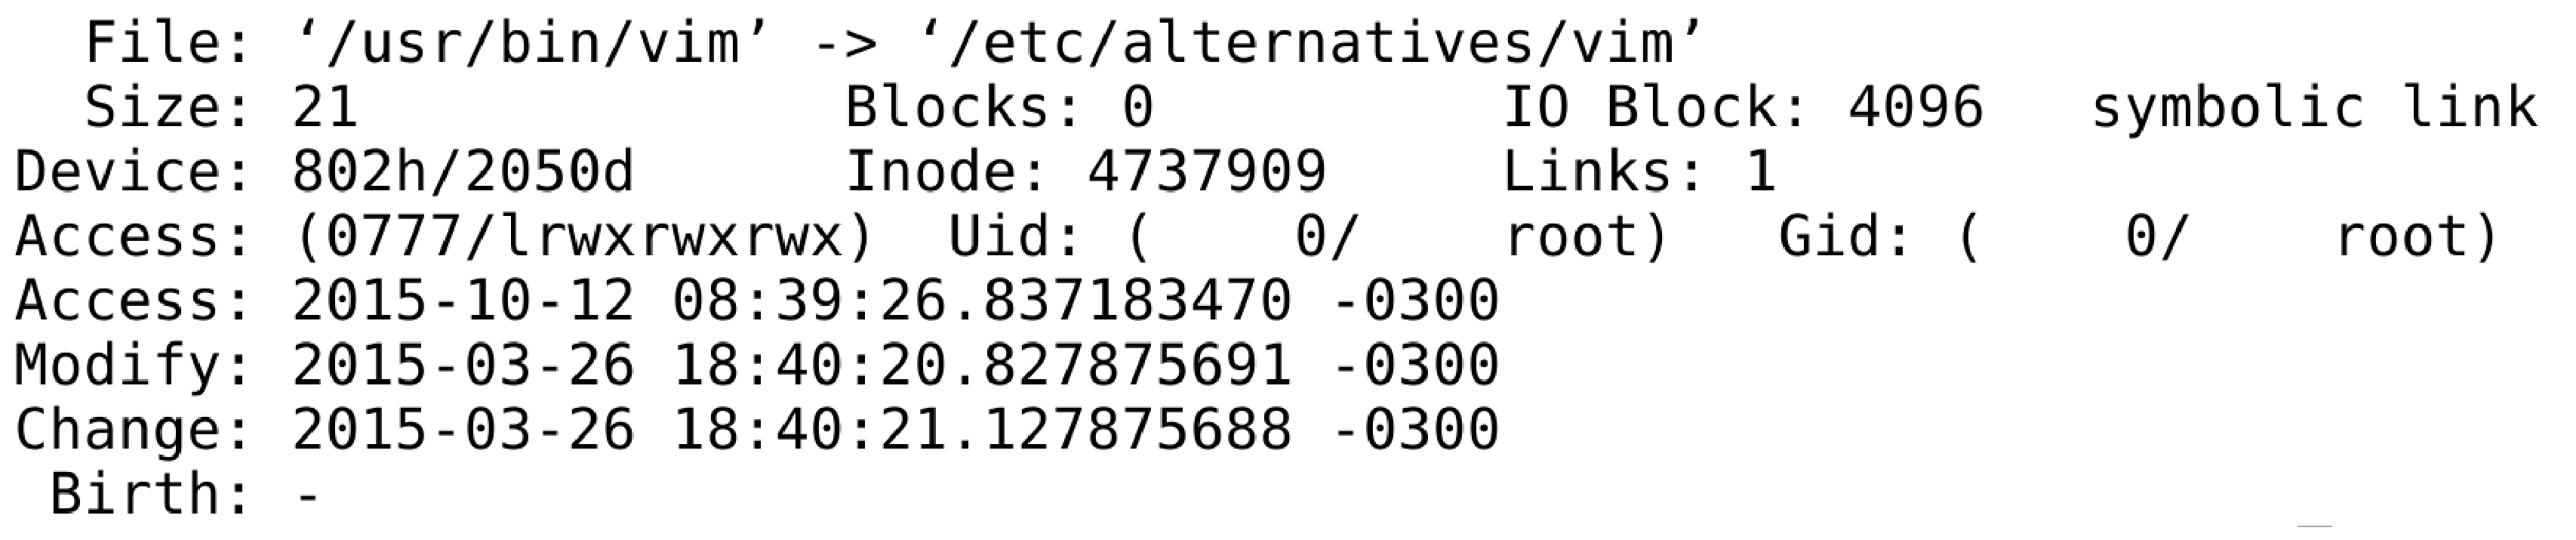
\includegraphics[width=1\textwidth]{figura/comando_stat.eps}
    \caption{Saída do comando stat para um dado software}
\end{figure}
\end{frame}


\begin{frame}
\begin{figure}[h!]
    \centering
    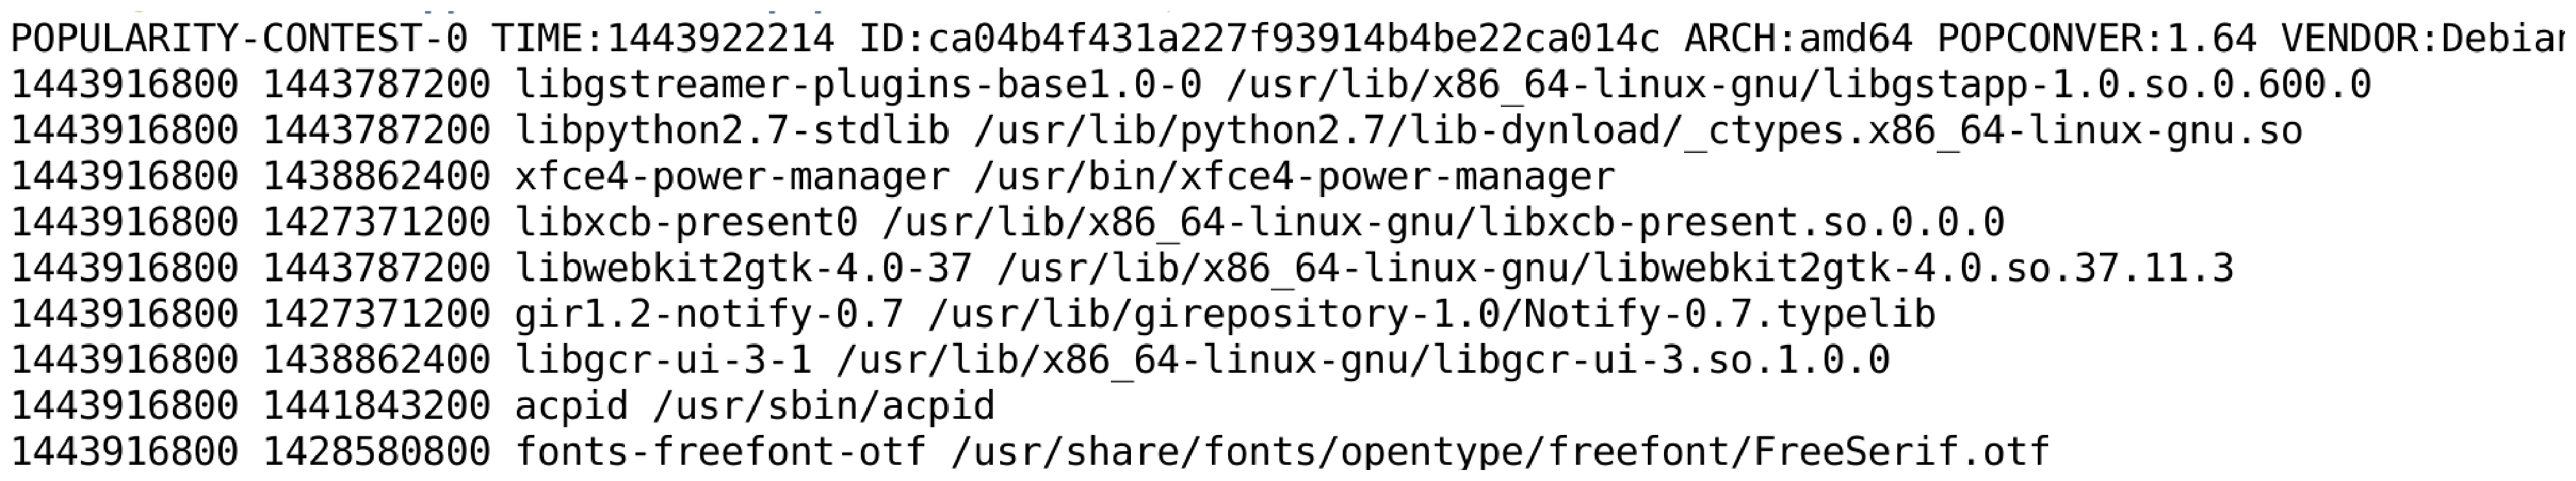
\includegraphics[width=1\textwidth]{figura/popularity_contest.eps}
    \caption{Saída do popularity-contest para um dado usuário}
\end{figure}
\end{frame}


\begin{frame}

    Atributos utilizados para se classificar um pacote através
    de um contexto temporal:

    \begin{itemize}
        \item \textbf{Tempo de Acesso:} Tempo de último acesso do pacote
        em segundos.

        \item \textbf{Tempo de Modificação:} Tempo de última modificação
        do pacote em segundos.

        \item \textbf{Tempo Atual:} Tempo atual no qual o usuário executa
        a aplicação.
    \end{itemize}

\end{frame}


\begin{frame}

    Através desses três atributos um pacote é clássificado analisando
a seguinte relação

    \begin{figure}[h]
      \centering
      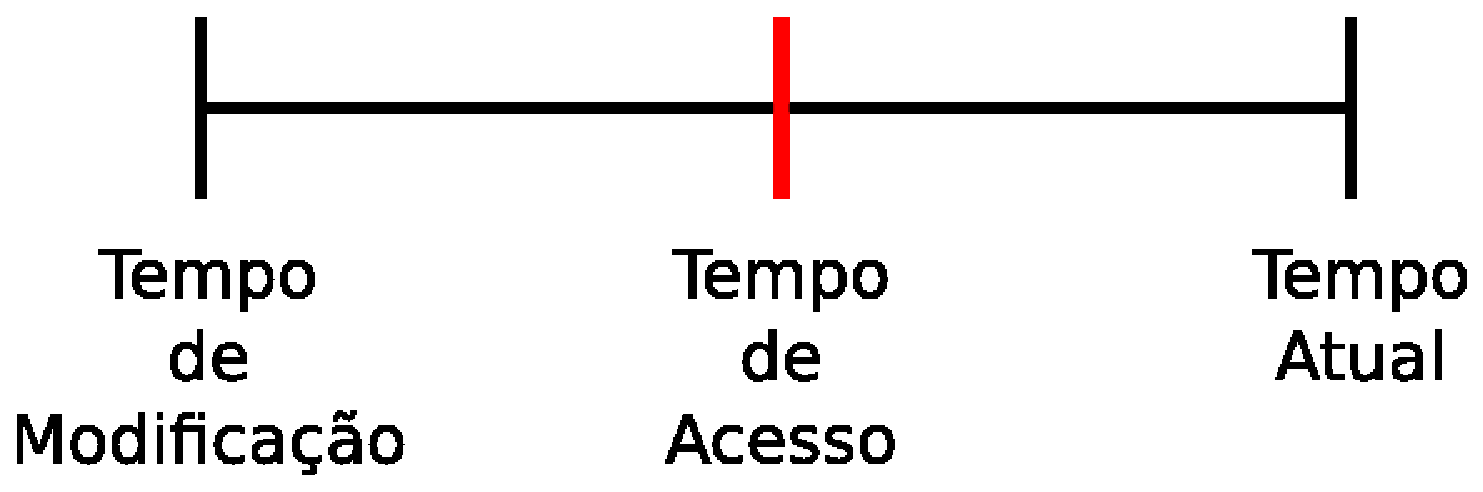
\includegraphics[width=0.9\textwidth]{figura/barra_temporal_01.eps}
      \caption{Classificação de um pacote no tempo}
      \label{fig:barra_temporal}
    \end{figure}

\end{frame}


\begin{frame}

    Quanto mais o Tempo de Acesso estiver próximo do Tempo Atual
melhor será a classificação de um pacote.
    \begin{figure}[h]
      \centering
      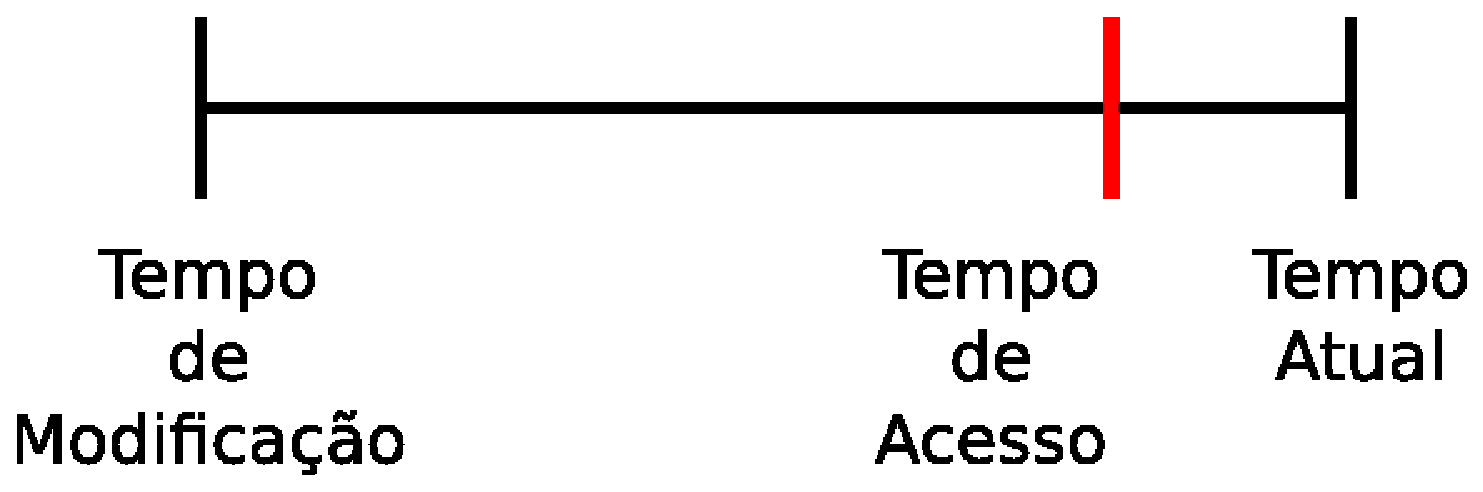
\includegraphics[width=0.9\textwidth]{figura/barra_temporal_02.eps}
      \caption{Classificação de um pacote no tempo}
      \label{fig:barra_temporal}
    \end{figure}

\end{frame}


\begin{frame}

    Quanto mais o Tempo de Acesso estiver próximo do Tempo de Modificação
pior será a classificação de um pacote.
    \begin{figure}[h]
      \centering
      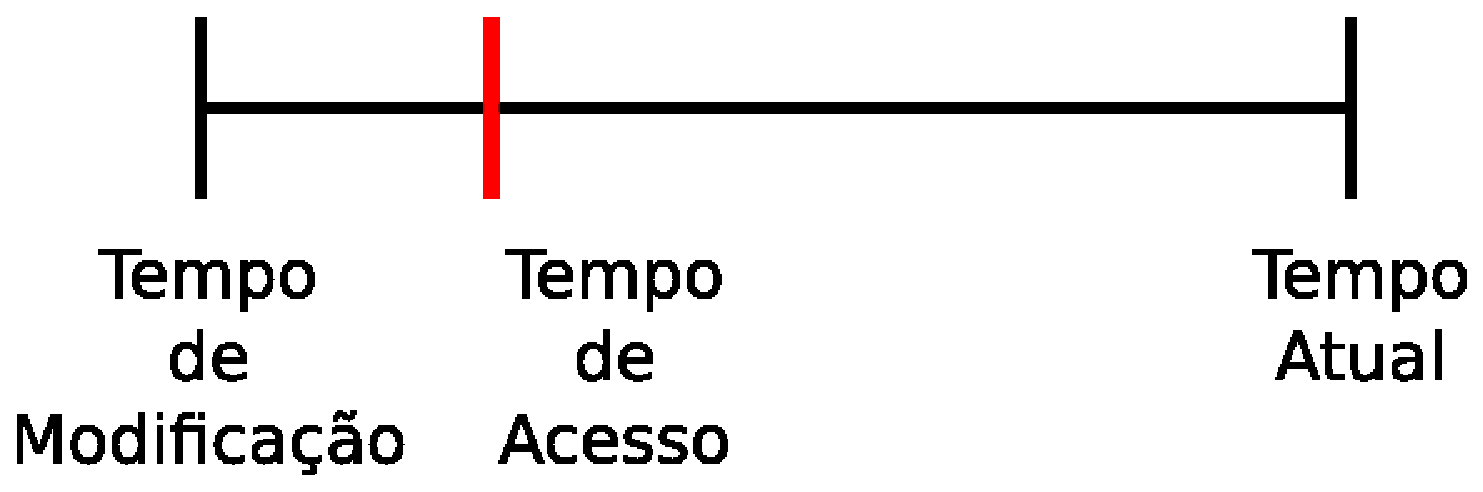
\includegraphics[width=0.9\textwidth]{figura/barra_temporal_03.eps}
      \caption{Classificação de um pacote no tempo}
      \label{fig:barra_temporal}
    \end{figure}

\end{frame}


\begin{frame}

    \begin{figure}[h]
      \centering
      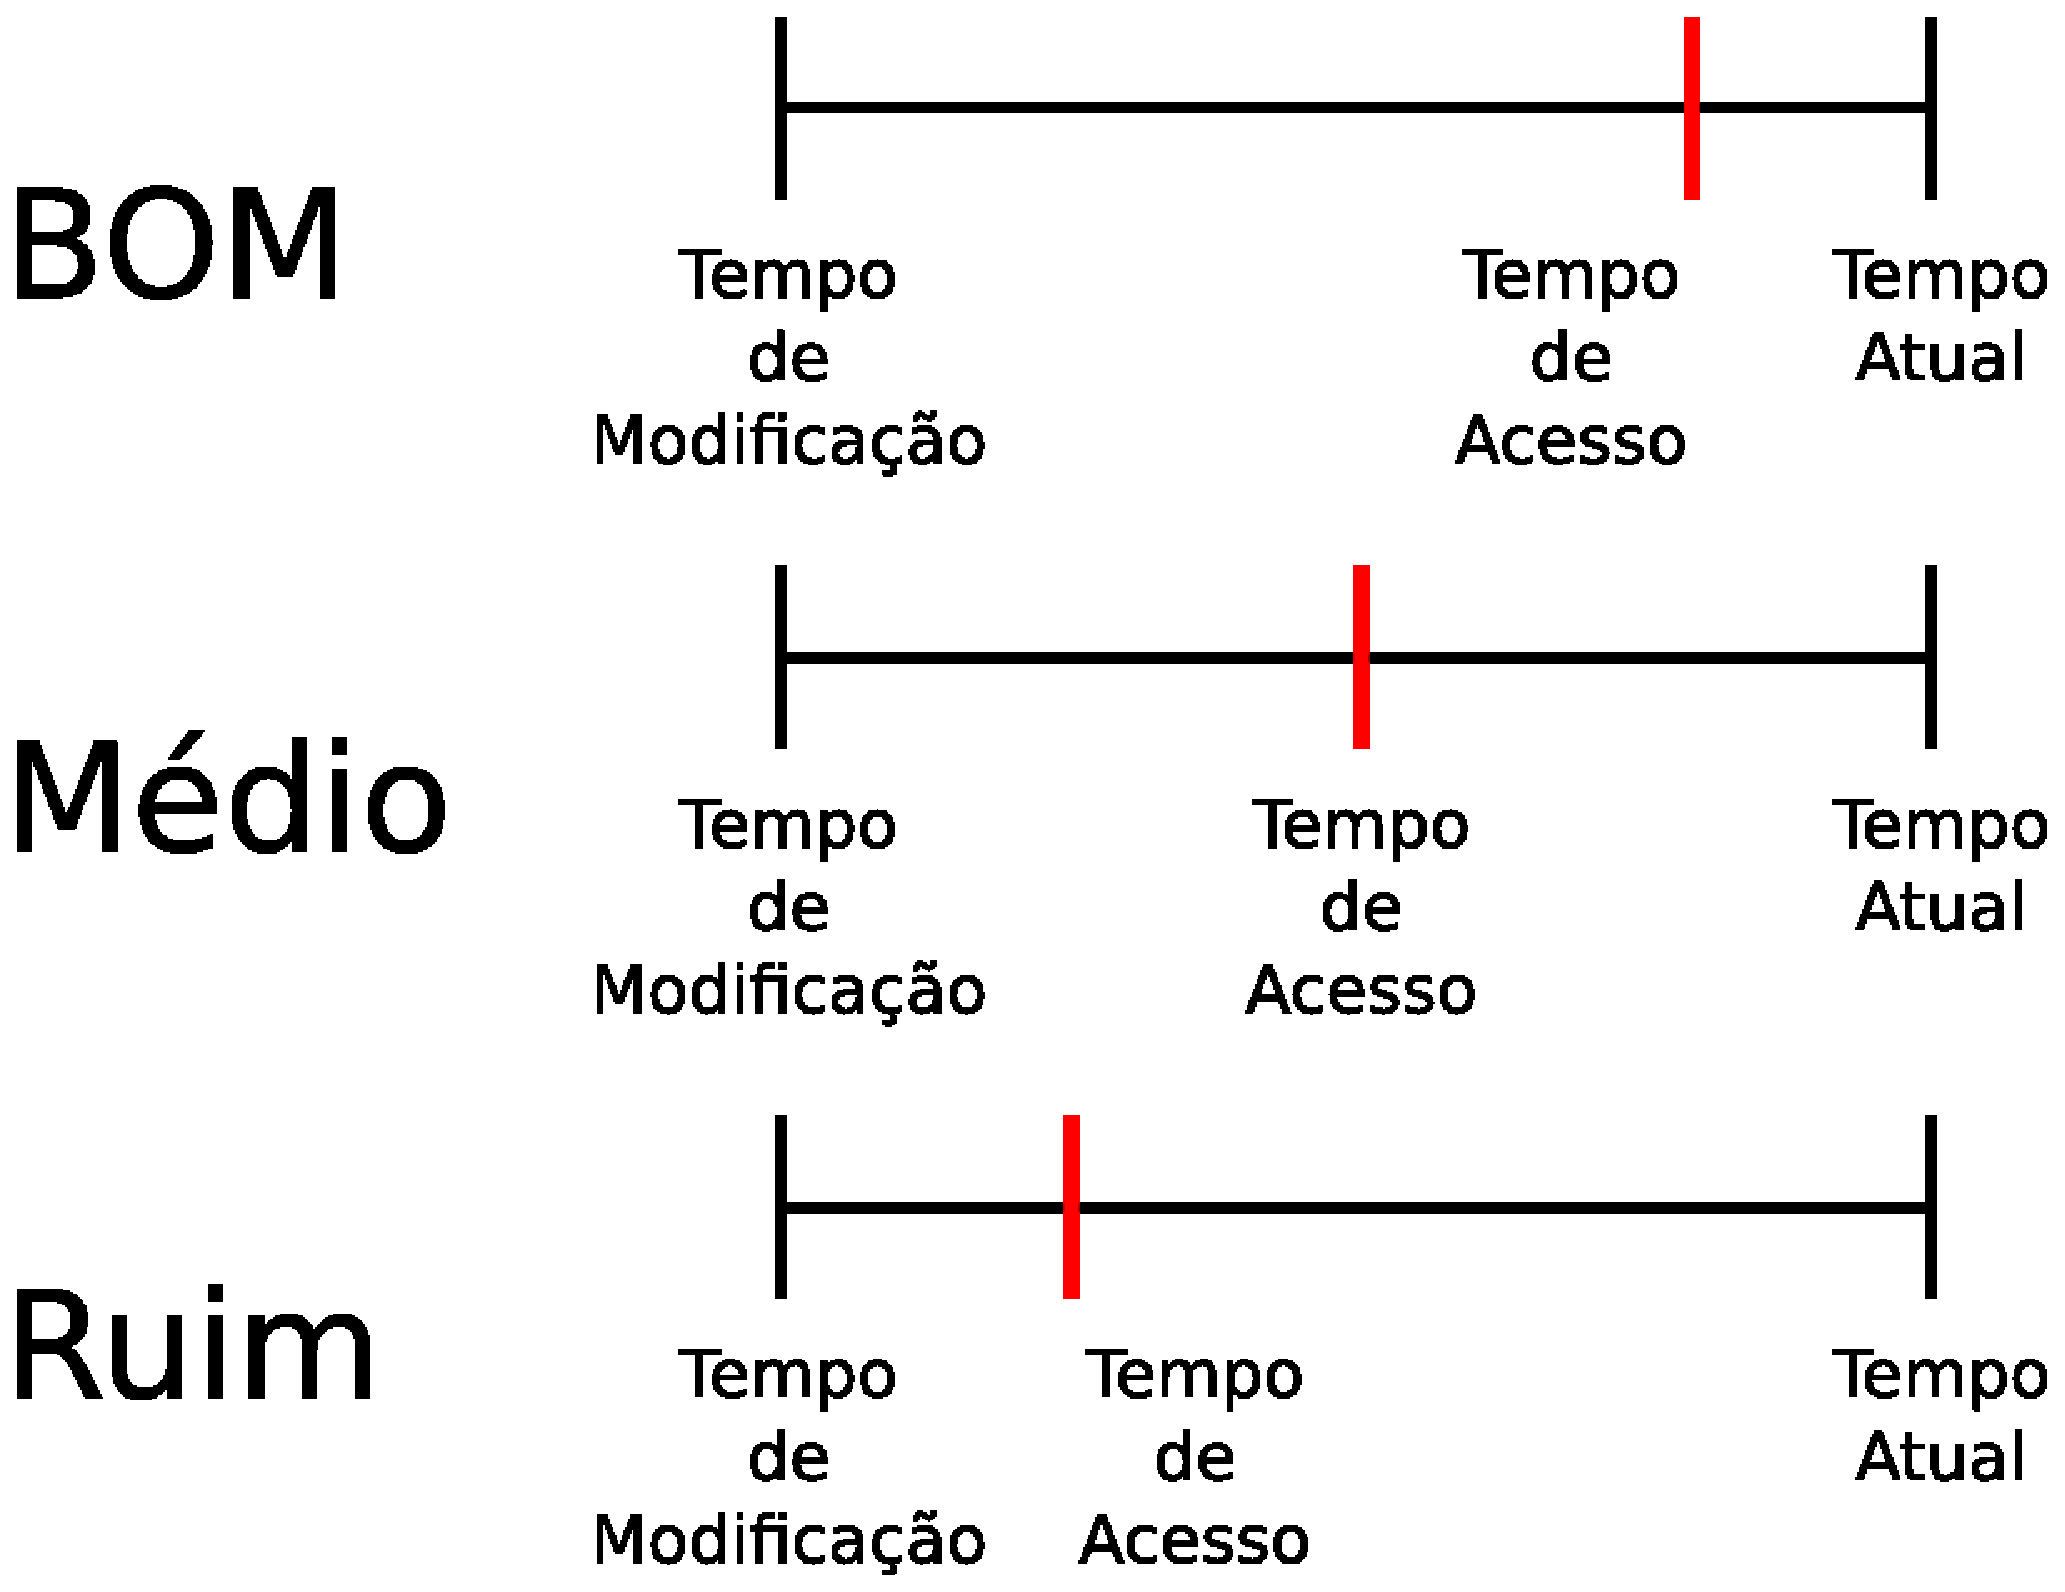
\includegraphics[width=0.9\textwidth]{figura/barra_temporal_04.eps}
      \caption{Classificação de um pacote no tempo}
      \label{fig:barra_temporal}
    \end{figure}

\end{frame}


\begin{frame}

    As imagens que demonstram a classificação temporal de um pacote
podem ser representada através da seguinte fórmula
    \newline
    \newline
    ClassificaçãoTemporal = $\frac{TempoAcesso - TempoModificação}{TempoAtual -
    TempoModificação}$

\end{frame}


\begin{frame}

    As imagens que demonstram a classificação temporal de um pacote
podem ser representada através da seguinte fórmula
    \newline
    \newline
    ClassificaçãoTemporal = $\frac{TempoAcesso - TempoModificação}{TempoAtual -
    TempoModificação}$
    \newline
    \newline
    Onde a classificação temporal de um pacote resulta em um valor
no intervalo de 0.0 a 1.0

    Quanto mais o resultado chegar perto do valor 1.0 melhor
é a classificação do pacote

\end{frame}


\begin{frame}
    Restrição quanto ao sistema de arquivo

    \begin{itemize}
        \item noatime
        \item stricatime
        \item relatime
    \end{itemize}
\end{frame}

\begin{frame}

    \begin{itemize}
        \item Pacotes usados sem intervenção direta do usuário
            \begin{itemize}
                \item Retirada de pacotes com prioridade \textit{Required},
                      \textit{Important} e \textit{Standard}.
            \end{itemize}
        \item Flag relatime não apresenta valores exatos
    \end{itemize}

\end{frame}

% section d (end)
\section{Estratégia determinística} % (fold)
\label{sec:estrategia_deterministica}

\begin{frame}
\begin{itemize}
    \item Usar uma fórmula para criação do perfil de usuário utilizando
    o contexto temporal
\end{itemize}
\end{frame}

\begin{frame}
\begin{itemize}
    \item Modifica o cálculo do peso dos pacotes em uma estratégia
    baseada em conteúdo
    \item O peso do pacote é resultado do produto do TFIDF com o
    Peso Temporal do pacote
\end{itemize}
\end{frame}

\begin{frame}
    Cada termo possui pacotes associados a ele:
    \begin{itemize}
        \item termo: role::program
        \item pacotes associados: vim, nano, git, gedit, python, inkscape
    \end{itemize}
\end{frame}

\begin{frame}
    \begin{itemize}
        \item Cada pacote possui um valor pela classificação temporal.
        \item Utilza-se do decaímento exponencial para controlar a suavidade da
curva que trata o peso do pacote.
    \end{itemize}

    \begin{figure}[h]
      \centering
      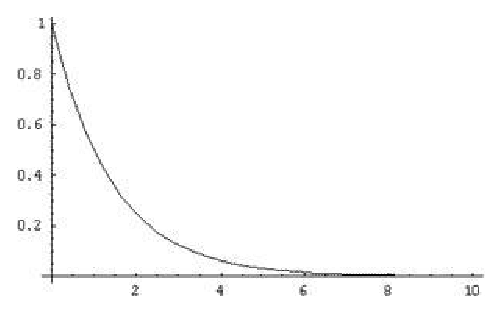
\includegraphics[width=0.9\textwidth]{figura/decaimento_exponencial.eps}
      \caption{Exemplo de um decaímento exponencial}
      \label{fig:curva_aprendizado}
    \end{figure}
\end{frame}

\begin{frame}
\begin{itemize}
    \item \textbf{PesoPacote} = $\frac{C}{\exp\left(({ClassificaçãoTemporal - 1}) * {\lambda}\right)}$
    \item Onde C e ${\lambda}$ são constantes usadas para alterar a velocidade do
decaimento da curva e o peso dado a variável \textit{ClassificaçãoTemporal}.
\end{itemize}
\end{frame}

\begin{frame}
    \begin{itemize}
        \item O peso de um termo é calculado pela média aritimética dos cinco
pacotes com maiores pesos que estão associados
ao termo.
        \item Termo: role::program
        \item Pacotes: vim, nano, git, gedit, python, inkscape
    \end{itemize}
    \begin{table}[h]
    \centering
    \begin{tabular}{cccccc}
    \hline
    \rowcolor[HTML]{EFEFEF}
    {vim} & {nano} & {git} & {gedit} & {python} & {inkscape} \\ \hline
    {5} & {2} & {4} & {3} & {2} & {1} \\ \hline
    \end{tabular}
    \caption{Exemplo de peso dos pacotes}
    \label{tab:classificacao_pacotes}
    \end{table}
\end{frame}

\begin{frame}
    \begin{itemize}
        \item O peso de um termo é calculado pela média aritimética dos cinco
pacotes com maiores pesos que estão associados
ao termo.
        \item Termo: role::program
        \item Pacotes: vim, nano, git, gedit, python, inkscape
    \end{itemize}
    \begin{table}[h]
    \centering
    \begin{tabular}{cccccc}
    \hline
    \rowcolor[HTML]{EFEFEF}
    {\textcolor{red}{vim}} & {\textcolor{red}{nano}} & {\textcolor{red}{git}} & {\textcolor{red}{gedit}} & {\textcolor{red}{python}} & {inkscape} \\ \hline
    {5} & {2} & {4} & {3} & {2} & {1} \\ \hline
    \end{tabular}
    \caption{Exemplo de peso dos pacotes}
    \label{tab:classificacao_pacotes}
    \end{table}
\end{frame}

\begin{frame}
    \begin{itemize}
        \item O valor temporal de um termo é calculado pela média aritimética dos cinco
pacotes com maiores pesos que estão associados
ao termo.
        \item Termo: role::program
        \item Pacotes: vim, nano, git, gedit, python, inkscape
    \end{itemize}

    $ValorTemporalDoTermo = \frac{5 + 4 + 3 + 2 + 2}{5}$
\end{frame}

\begin{frame}
    \begin{itemize}
        \item O valor temporal de um termo é calculado pela média aritimética dos cinco
pacotes com maiores pesos que estão associados
ao termo.
        \item Termo: role::program
        \item Pacotes: vim, nano, git, gedit, python, inkscape
    \end{itemize}

    $ValorTemporalDoTermo = 3.2$
\end{frame}

\begin{frame}
    \begin{itemize}
        \item O valor temporal de um termo é calculado pela média aritimética dos cinco
pacotes com maiores pesos que estão associados
ao termo.
        \item Termo: role::program
        \item Pacotes: vim, nano, git, gedit, python, inkscape
    \end{itemize}

    $ValorTemporalDoTermo = 3.2$
    $PesoDoTermo = TFIDF * ValorTemporalDoTermo$
\end{frame}

\begin{frame}
    \begin{itemize}
        \item Caso o termo possua menos de 5 pacotes os valores faltantes são
    preenchidos pelo peso anterior com um decréscimo de 0.05
        \item Termo: role::program
        \item Pacotes: vim, nano
    \end{itemize}

    \begin{table}[h]
    \centering
    \begin{tabular}{cccccc}
    \hline
    \rowcolor[HTML]{EFEFEF}
    {vim} & {nano} & {X} & {X} & {X} \\ \hline
    {5.0} & {2.0} & {1.95} & {1.90} & {1.85} \\ \hline
    \end{tabular}
    \caption{Exemplo de peso dos pacotes}
    \label{tab:classificacao_pacotes}
    \end{table}
\end{frame}

\begin{frame}
    \begin{itemize}
        \item Caso o termo possua menos de 5 pacotes os valores faltantes são
    preenchidos pelo peso anterior com um decréscimo de 0.05
        \item Termo: role::program
        \item Pacotes: vim, nano
    \end{itemize}

    $ValorTemporalDoTermo = \frac{5.0 + 2.0 + 1.95 + 1.90 + 1.85}{5}$
\end{frame}

\begin{frame}
    \begin{itemize}
        \item Caso o termo possua menos de 5 pacotes os valores faltantes são
    preenchidos pelo peso anterior com um decréscimo de 0.05
        \item Termo: role::program
        \item Pacotes: vim, nano
    \end{itemize}

    $ValorTemporalDoTermo = 2.54$
\end{frame}

\begin{frame}
    \begin{itemize}
        \item Caso o termo possua menos de 5 pacotes os valores faltantes são
    preenchidos pelo peso anterior com um decréscimo de 0.05
        \item Termo: role::program
        \item Pacotes: vim, nano
    \end{itemize}

    $ValorTemporalDoTermo = 2.54$

    $PesoDoTermo = TFIDF * ValorTemporalDoTermo$
\end{frame}

\begin{frame}
    \begin{itemize}
        \item Os termos com os maiores pesos se tornam o perfil do usuário
    \end{itemize}
\end{frame}

% section d (end)

\section{Aprendizado de máquina} % (fold)

\begin{frame}

    \begin{itemize}
        \item Estratégia de pós-filtragem
        \item Rótulos do pacote
        \item Formatação dos dados
        \item Estratégia de aprendizado
    \end{itemize}

\end{frame}

\begin{frame}

    Rótulos do pacote:
    \newline
    \newline

    \begin{table}[h]
    \centering
    \begin{tabular}{cc}
    \hline
    \rowcolor[HTML]{EFEFEF}
    {Escala} & {Valores} \\ \hline
    {Excelent(EX)}  & ClassificaçãoTemporal >= 0.8                  \\ \hline
    {Great(G)}   & ClassificaçãoTemporal >= 0.7                  \\ \hline
    {Medium(M)}   & ClassificaçãoTemporal >= 0.5                  \\ \hline
    {Bad(B)}   & ClassificaçãoTemporal >= 0.3                  \\ \hline
    {Horrible(H)}   &ClassificaçãoTemporal < 0.3                   \\ \hline
    \end{tabular}
    \caption{Escala para classificação de um pacote baseado em seus atributos de tempo}
    \label{tab:classificacao_pacotes}
    \end{table}

\end{frame}

\begin{frame}

    \begin{itemize}
        \item Vetores binários em ordem alfabética para representar um pacote
        \item Debtags e descrição do pacote
        \item Termos usados apenas dos pacotes manualmente instalados pelo
              usuário
    \end{itemize}
\end{frame}

\begin{frame}
 \begin{figure}[h]
  \centering
  
\includegraphics[width=0.9\textwidth]{figura/vetor_binario.eps}
  \caption{Exemplo de vetor binário}
  \label{fig:curva_aprendizado}
 \end{figure}
\end{frame}

\begin{frame}

    \begin{itemize}
        \item Bayes ingênuo
        \item Uso da probabilidade de bayes
        \item Distribuição de Bernoulli
        \item Dependência entre variáveis não levada em conta
        \item Linearização do método
    \end{itemize}

\end{frame}

\begin{frame}

    Fórmula adotada para o bayes ingênuo:
    \newline
    \newline
    $Classificador = max(p(C_{y})*\prod_{i=1}^{N}p(x_{i}|C_{y}))$


    \begin{itemize}
        \item $NR$: Número total de rótulos
        \item $NC_{y}$: Número total de rótulos $C_{y}$
        \item $C_{y}$: Possível rótulo do pacote
        \item $p(C_{y})$: $NC_{y}/NR$
        \item $Nx_{i}C_{y}$: Número de vezes que $x_{i}$ esta presente em $C_{y}$
        \item $p(x_{i}|C_{y})$: $Nx_{i}C_{y}/NC_{y}$
    \end{itemize}


\end{frame}

\begin{frame}

    \begin{itemize}
        \item Validação cruzada
        \item Curvas de Aprendizado
    \end{itemize}

\end{frame}

\begin{frame}

\begin{figure}[h]
  \centering
  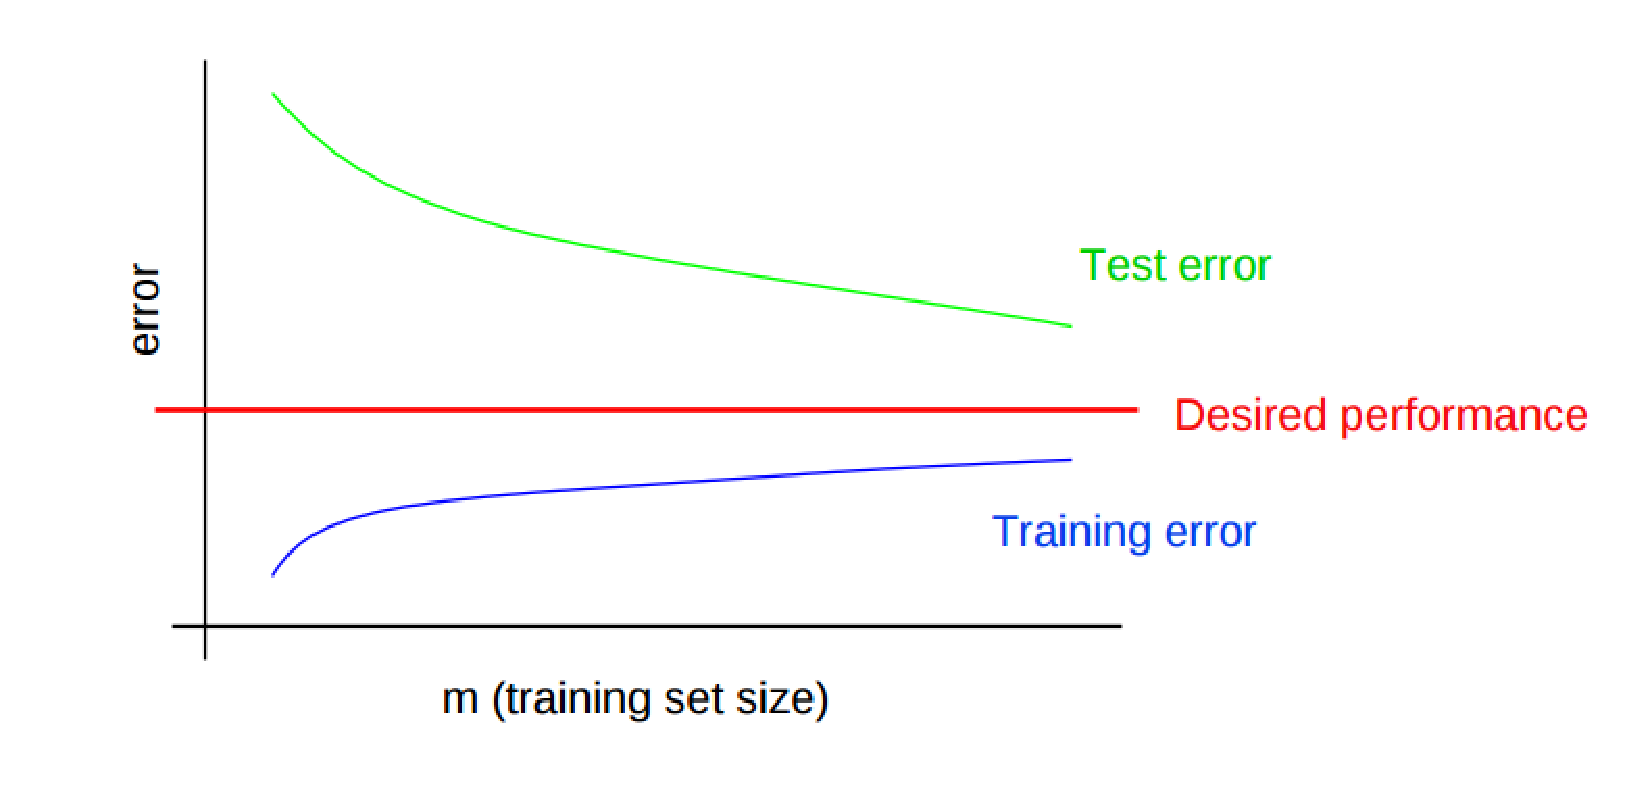
\includegraphics[width=0.9\textwidth]{figura/curva_aprendizado.eps}
  \caption{Exemplo de uma curva de aprendizado}
  \label{fig:curva_aprendizado}
\end{figure}

\end{frame}


\label{sec:aprendizado_maquina}

\section{Comparação dos resultados} % (fold)
\label{sec:comparacao_resultados}

\begin{frame}
    \begin{itemize}
        \item Comparação baseadas no \textit{AppRecommender}
        \item Foco em precisão e novidade das recomendações
        \item Comparação \textit{offline}
        \item Teste com usuário
        \item Coleta de dados para comparação \textit{offline}
    \end{itemize}
\end{frame}

\begin{frame}
\begin{figure}[h]
  \centering
  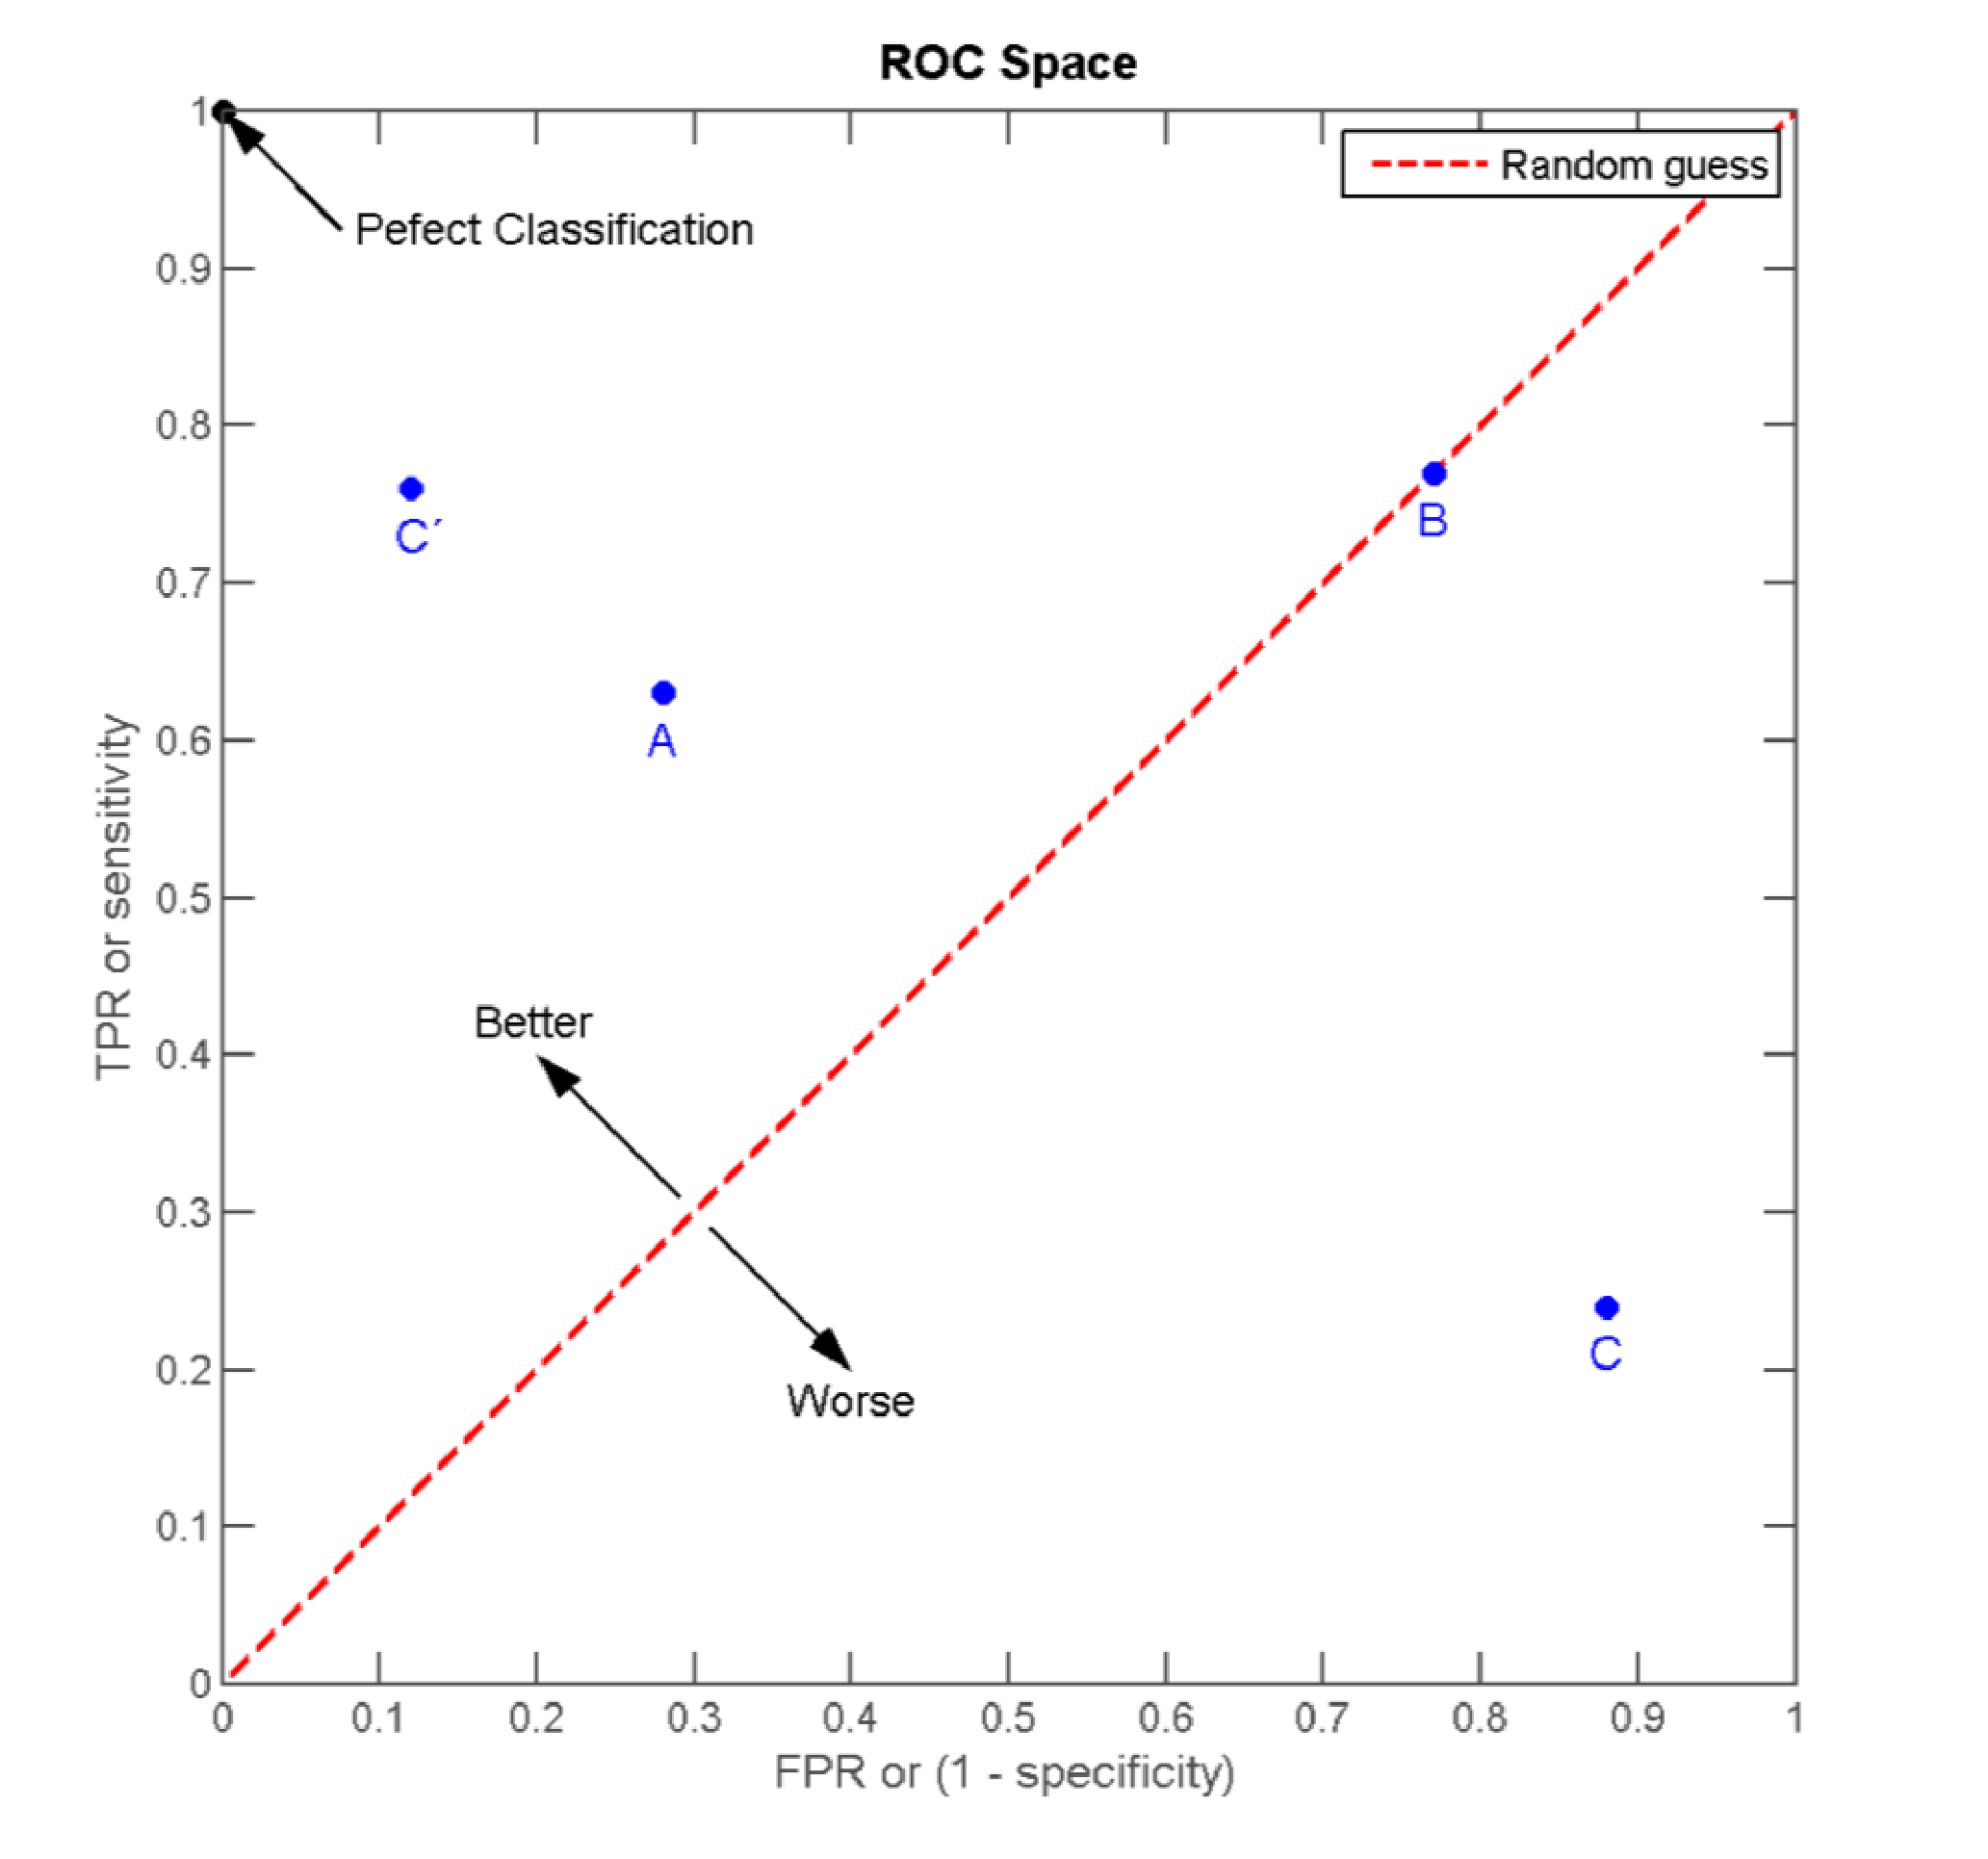
\includegraphics[width=0.7\textwidth]{figura/curva_roc.eps}
  \caption{Exemplo de curva ROC}
  \label{fig:curva_roc}
\end{figure}

\end{frame}

\begin{frame}

    \begin{itemize}
        \item Usuário será apresentado a 5 recomendações de cada vez
        \item 4 estratégias distintas
        \item 20 recomendações de pacotes no total
    \end{itemize}

\end{frame}

\begin{frame}

 \begin{itemize}
    \item \textbf{Ruim: } Recomendação que não agrada ao usuário.
    \item \textbf{Redundante: } Usuário possui aplicativos similares para o item
        sendo recomendado.
    \item \textbf{Útil: } Usuário acha que a recomendação lhe proporciona um
            pacote útil.
    \item \textbf{Surpresa boa: } Usuário considera a recomendação útil e além
        do mais inesperada.
\end{itemize}


\end{frame}

\begin{frame}

\begin{itemize}
    \item \textbf{Precisão: } $\frac{VerdadeirosPositivos}{VerdadeirosPositivos
        + FalsoNegativos}$
    \item \textbf{Novidade: } $\frac{NumSurpresaBoa}{VerdadeirosPositivos +
        FalsoNegativos}$
\end{itemize}

Onde:

    \begin{itemize}
        \item VerdadeirosPositivos: Útil e Surpresa boa
        \item FalsoNegativos: Ruim e Redundante
    \end{itemize}

\end{frame}

\section{Resultados parciais} % (fold)
\label{sec:resultados_parciais}

\begin{frame}
\begin{itemize}
    \item AppRecommender
    \item Coleta das informações temporais dos pacotes
    \item Estratégia determinística
    \item Aprendizado de máquina: A técnica está implementada.
    Coleta de dados dos pacotes, extrair seus atributos e classificá-los.
    \item Coleta de dados dos usuários
\end{itemize}
\end{frame}

\section{Obrigado!}
\label{sec:obrigado}


